\documentclass[11pt]{beamer}

\usetheme{epfl}
\usepackage{tikz}

\usepackage{pgfplots}
\pgfplotsset{compat=1.16}


\usetikzlibrary{positioning,arrows.meta}
\usetikzlibrary{calc,patterns,angles,quotes, fadings}
\usetikzlibrary{decorations,fit}

\usepackage{media9}
\usepackage{amsmath}
\usepackage[thicklines]{cancel}
\usepackage{svg}
\newcommand{\citeapa}[1]{ {\tiny#1\par} }
%\usepackage{utf8}
%\usepackage{fontspec}
\usepackage{booktabs}
\usepackage{multirow}
\usepackage{tumcolors}
\usepackage[ruled,vlined]{algorithm2e}
\usepackage{algorithmic}

% primary colors
%\definecolor{tumblue}{RGB}{0,101,189} % Pantone 300
%\definecolor{tumorange}{RGB}{227,114,34} % Pantone 158 - Orange
\setbeamercovered{transparent}

\colorlet{mamlcolor}{rouge}
\colorlet{pretrainedcolor}{taupe}
\colorlet{randomcolor}{acier}

\usepackage[eulergreek]{sansmath}
\pgfplotsset{
	y tick label style={/pgf/number format/.cd,scaled y ticks = false,set thousands separator={},fixed},
	tick label style = {font=\sansmath\sffamily\footnotesize},
	every axis label = {font=\sansmath\sffamily\scriptsize},
	every axis/.append style={axis lines=left, thick},
	legend style = {font=\sansmath\sffamily\scriptsize, draw=white, fill opacity=.5, text opacity=1},
	label style = {font=\sansmath\sffamily\footnotesize},
	grid style={line width=.1pt, draw=gray!10},
	major grid style={line width=.2pt,draw=perle},
	title style={font=\sansmath\sffamily},
	grid=both,
}


\begin{document}
	
	\title{Data-Driven Vegetation Modeling and Understanding Representation Shift}
	\subtitle{with Few-Shot Meta-Learning}
	\author{Marc Ru\ss{}wurm}
	\labname{EPFL-ECEO}
	\date{November 10th, 2021}
	
	\logofilename{epfl/epfl_red.png}
	\titlepageimage{epfl/lacleman}
	\event{Deep Learning for Environment}
	\presentation{Representation Shift and Few-Shot Meta-Learning}
	\speaker{Marc Russwurm}
	
	\begin{frame}[plain]
		\maketitle
	\end{frame}

%	\begin{frame}{Structure}
%		
%		\begin{enumerate}
%			\item Data-Driven Vegetation Modeling and 
%			\begin{itemize}
%				\item why is it meaningful
%				\item data-driven verus model-driven approaches
%			\end{itemize}
%			\item<2-> Tackling Representation Shift 
%			\begin{itemize}
%				\item when does it arise?
%				\item regional representations
%			\end{itemize}
%			\item<3> with Few-Shot Meta-Learning Methods
%			\begin{itemize}
%				\item seeing our remote sensing data as a dataset-of-datasets
%				\item Model-agnostic meta-learning as one algorithm to tackle it.
%			\end{itemize}
%		\end{enumerate}
%	
%	\end{frame}

%	\begin{frame}[plain]
%		\centering
%		\hfill
%		\Large
%		
%			Why do we need Vegetation Modeling?
%			\\
%			What do we measure?
%			\\
%			What data do we have available?
%			
%			
%		\hfill
%	\end{frame}

	\begin{frame}
		\frametitle{Why do we need Vegetation Modeling?}
		\begin{columns}
			\column{.5\textwidth}
			{\scriptsize
			\begin{description}
				\item[Zero Hunger] estimating the \textbf{crop yield} \& predict \textbf{food prices}, shortages.
				\item<2->[Climate Action] by monitoring \textbf{vegetation changes} over time (desertification).
				\item<3->[Life on Land] human life depends on \textbf{agriculture}, animal life on \textbf{biotopes}.
				%				\item Precision agriculture: sd
			\end{description}
			}
			\column{.5\textwidth}
			
\includegraphics[width=\textwidth]{images/sdg_goals.pdf}
			
		\end{columns}
	
		
	
		\only<4>{
			
			\vspace{2em}
			
			Crop Type Mapping:
			
			\vspace{1em}
			
			Satellite Time Series Data $\rightarrow$ Crop Type Label {\scriptsize (e.g. corn, meadow)}
		
	}
	\only<5>{	
			\vspace{2em}
			
			
			Later: Land Cover Classification
			
			\vspace{1em}
			Satellite Image $\rightarrow$ Land Cover Label \scriptsize (e.g. urban, forest)
			}
		
		
	\end{frame}


	\begin{frame}<presentation:1>
		\frametitle{Satellite Time Series $\rightarrow$ Crop Type}
		
		\begin{tikzpicture}[node distance=0em]
		\node(a) at (0,0){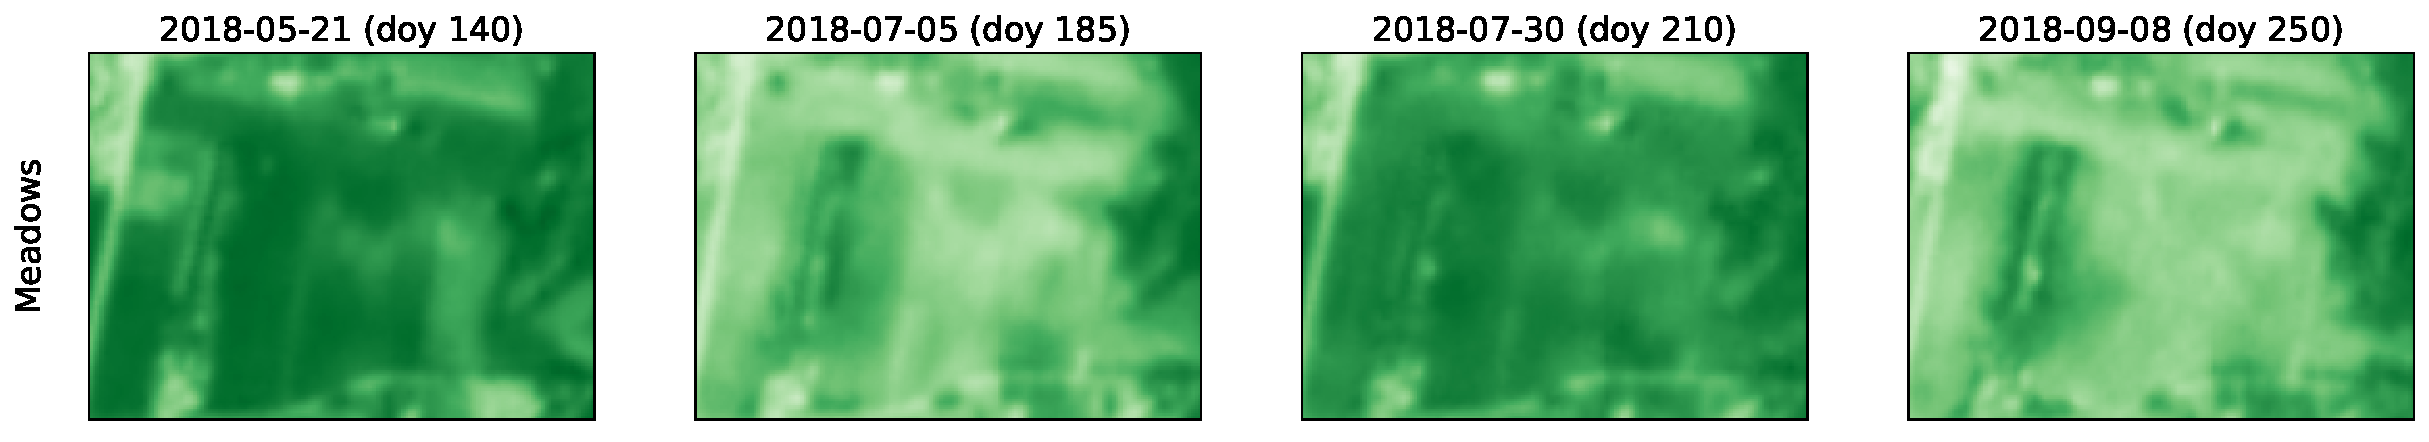
\includegraphics[width=10cm]{images/denethor/43647_Meadows_images}};
		\node(b)[below=0em of a]{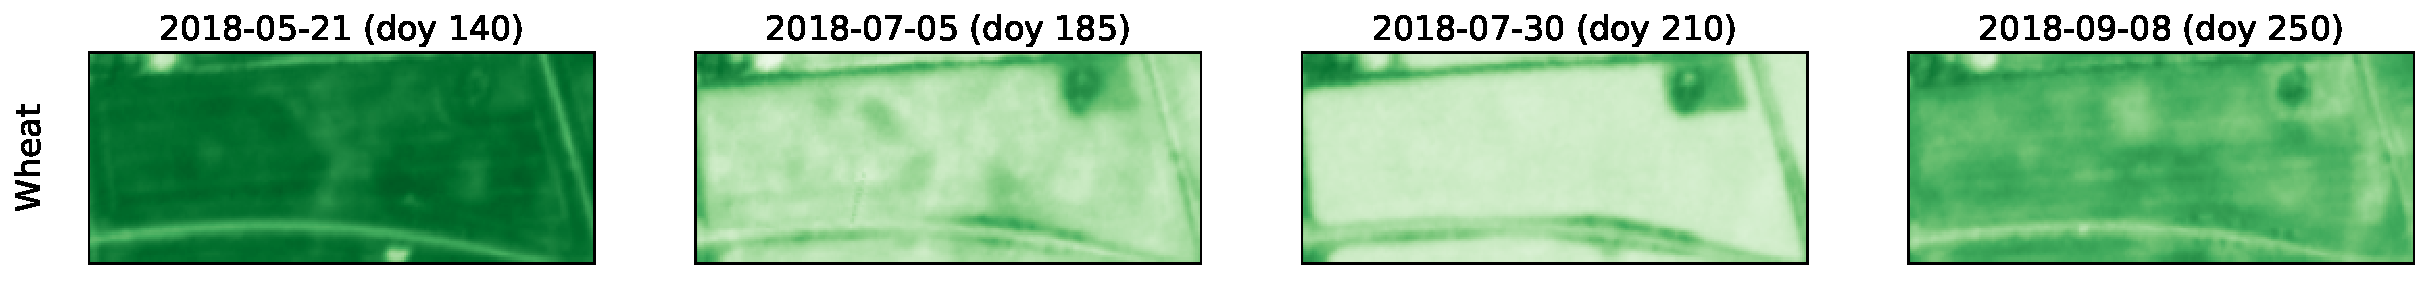
\includegraphics[width=10cm]{images/denethor/82235_Wheat_images}};
		\visible<1>{
			\node(c)[below=1cm of b, xshift=-4em]{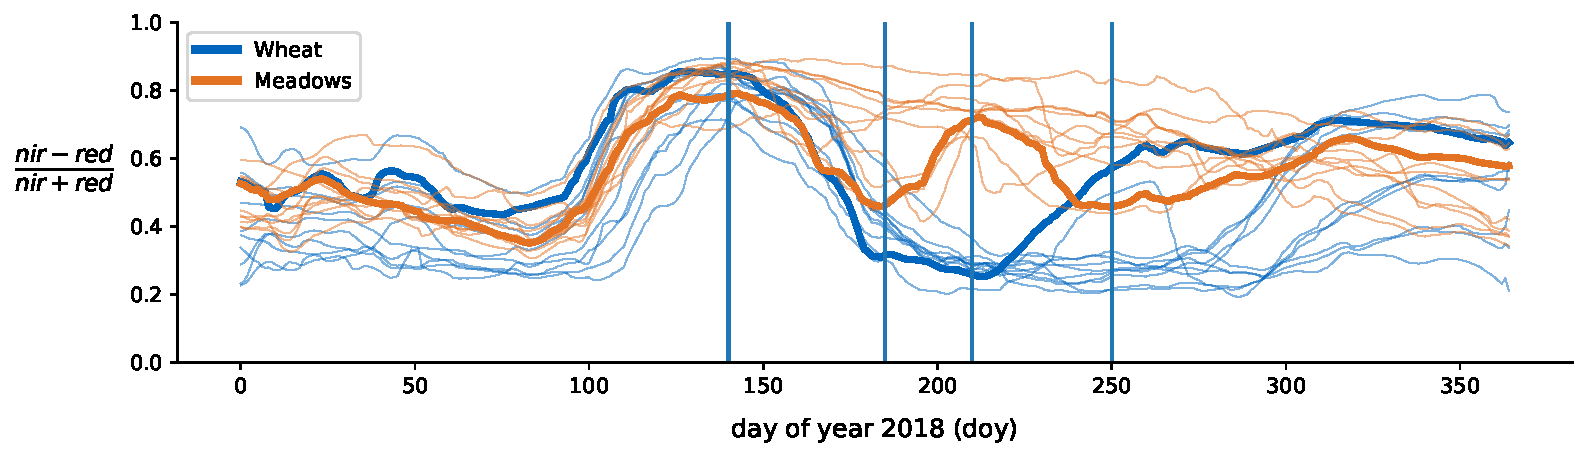
\includegraphics[width=.8\textwidth]{images/denethor/plots_2018.pdf}};
		}
		
		\visible<2>{
			\node(c)[below=1cm of b, xshift=-4em]{\includegraphics[width=.8\textwidth]{images/denethor/plotss2.pdf}};
		}
		\node(d)[right=-2em of c, yshift=1em]{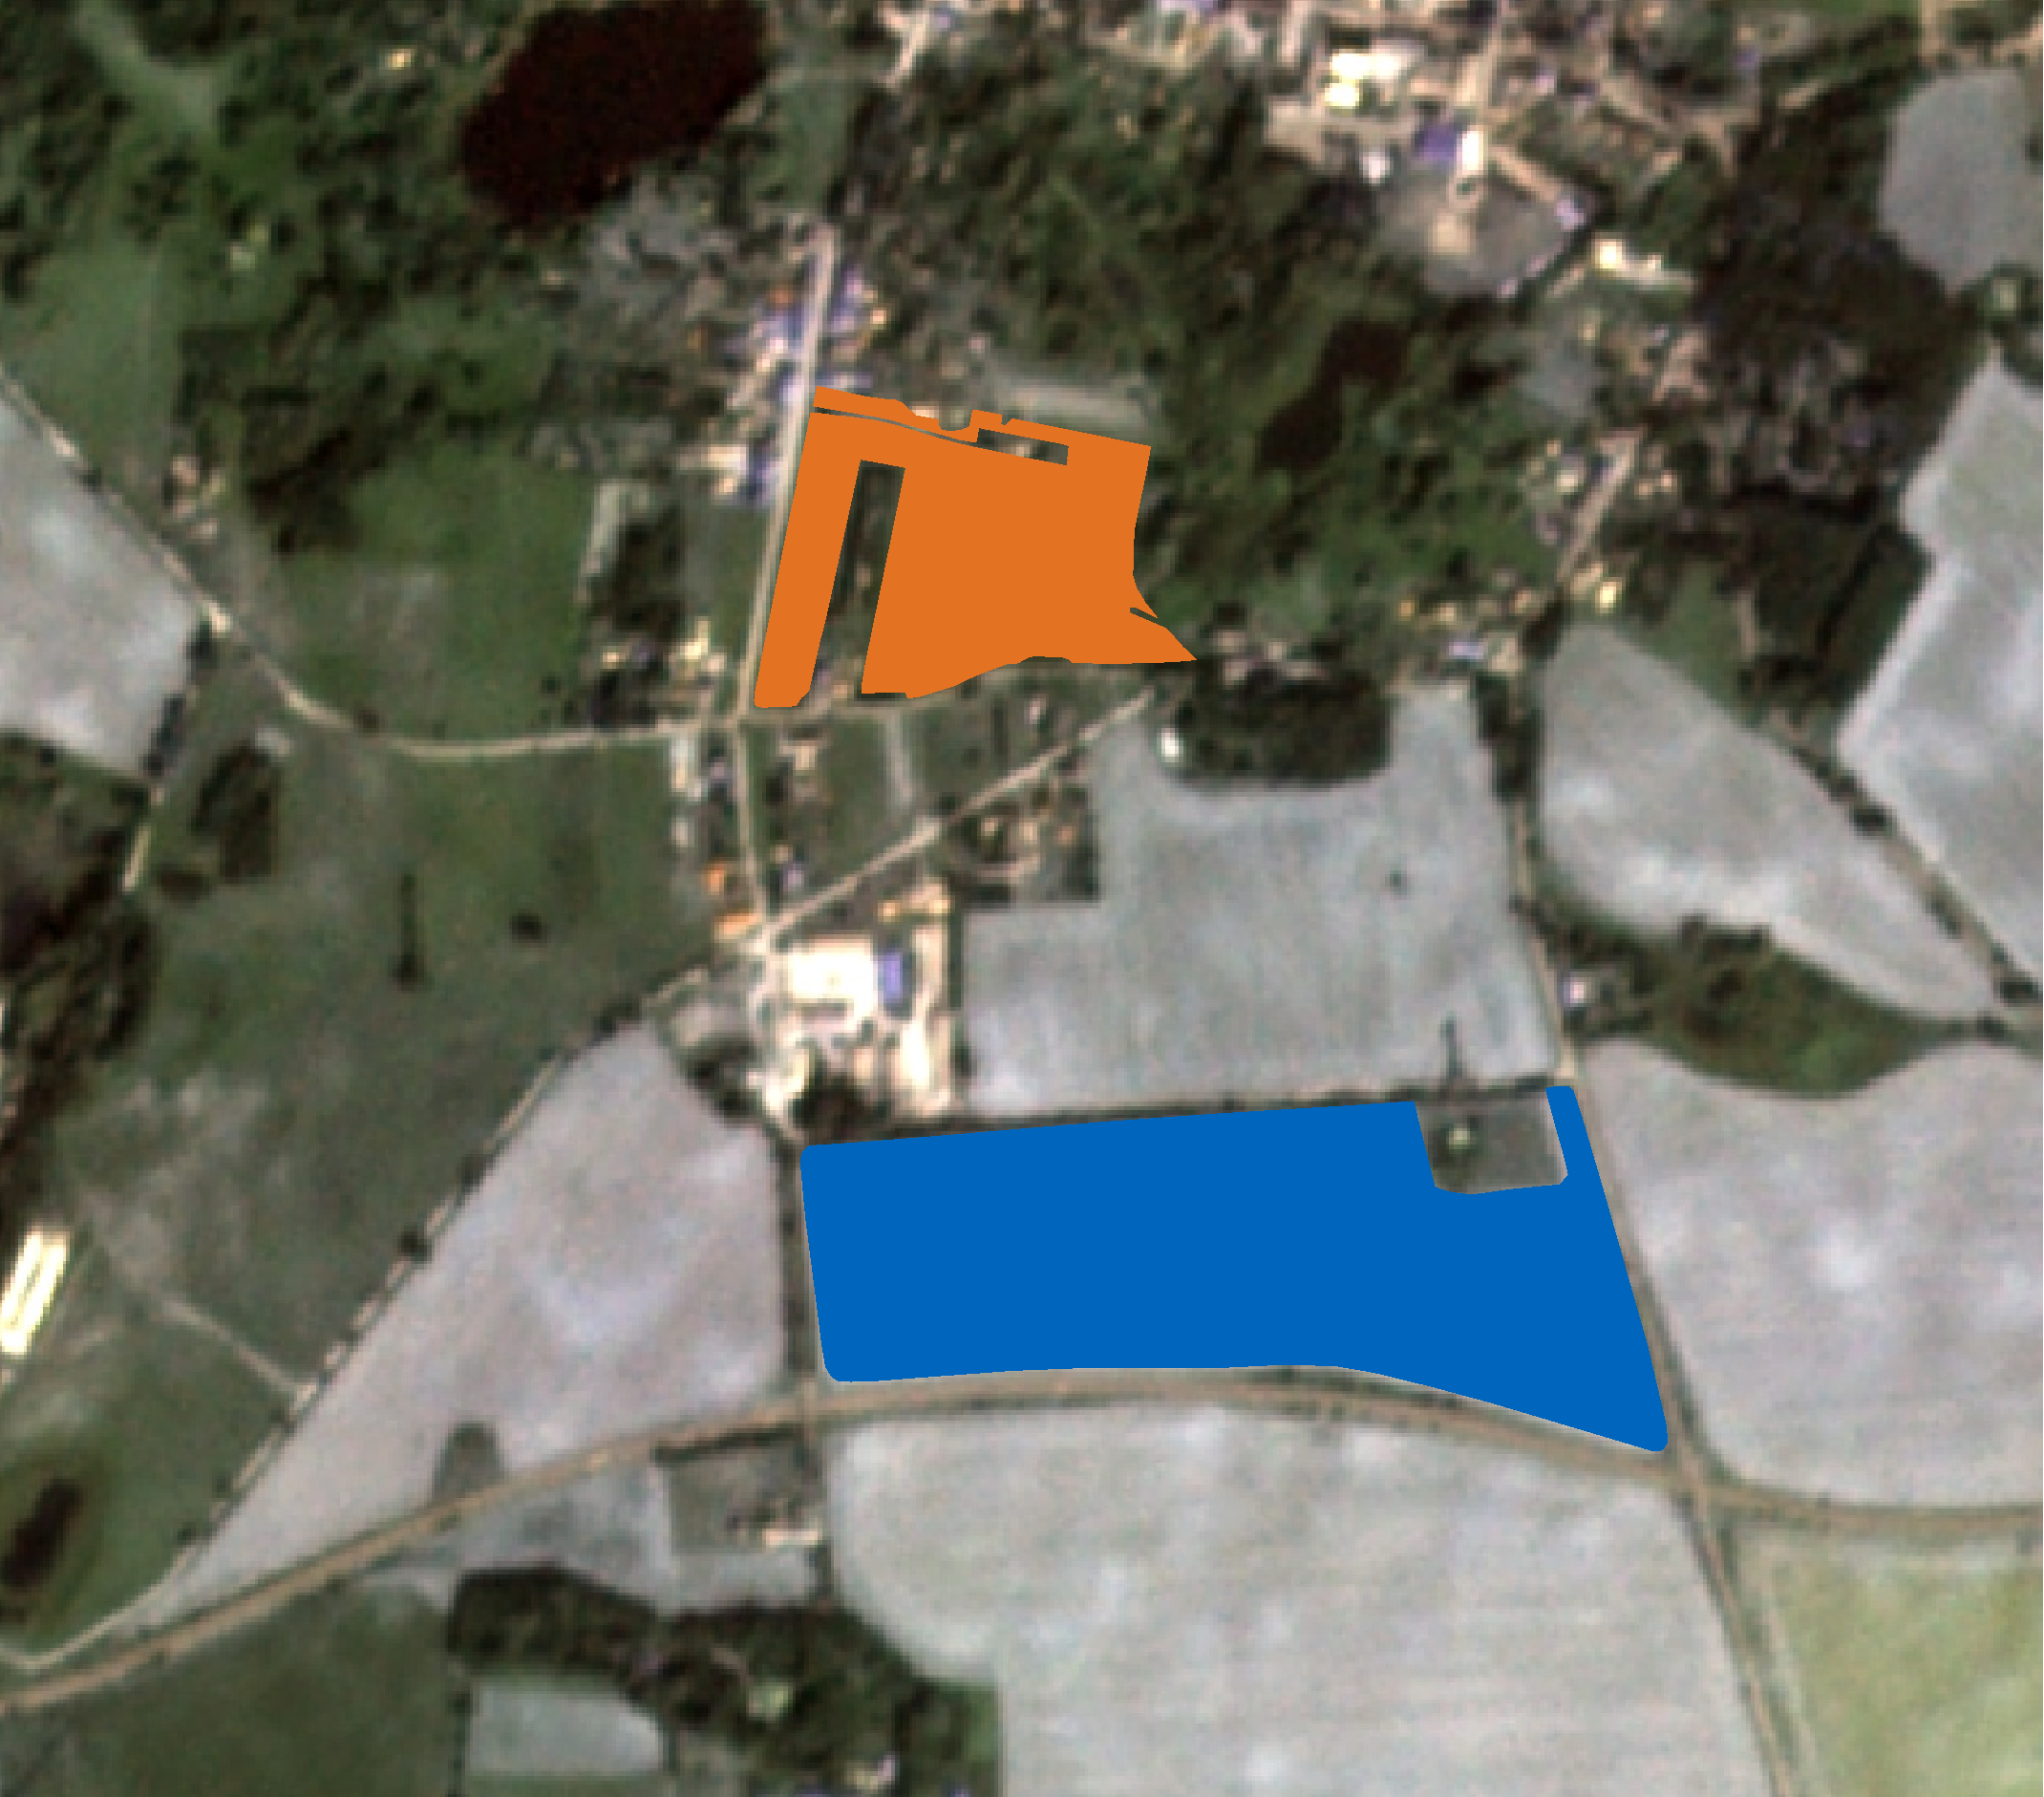
\includegraphics[width=3cm]{images/denethor/map}};
		
		%\node[below=of c]{\includegraphics[width=.9\textwidth]{images/plotss2}};
		
		\definecolor{mpldefaultblue}{HTML}{1f77b4}
		%\coodinate (l1) at ($ (c) + (1,1) $);
		%		\draw[Circle - , color=mpldefaultblue] ($ (c) + (-.45,1.6) $) -- ($ (b) + (-3.8,-.8) $); % requires \usetikzlibrary{arrows.meta} and calc
		%		\draw[Circle - , color=mpldefaultblue] ($ (c) + (.78,1.6) $) -- ($ (b) + (-1.4,-.8) $);
		%		\draw[Circle - , color=mpldefaultblue] ($ (c) + (1.38,1.6) $) -- ($ (b) + (1.6,-.8) $);
		%		\draw[Circle - , color=mpldefaultblue] ($ (c) + (2.46,1.6) $) -- ($ (b) + (5,-.8) $);
		
		%\node[circle, draw] at (l1) {+};
		
		\end{tikzpicture}
		
		\citeapa{Kondmann, et al., "DENETHOR: The DynamicEarthNET dataset for Harmonized, inter-Operable, analysis-Ready, daily crop monitoring from space.". NeurIPS Data Track (2021).}
	\end{frame}

	\begin{frame}{Satellite Time Series Data in Abundance}
		
%		\includemedia[
%		width=\textwidth,
%		activate=pageopen,
%		addresource=mp4/apenne_modis_ndvi.mp4,
%		flashvars={source=mp4/apenne_modis_ndvi.mp4&loop=true&
%			autoPlay=true}
%		]{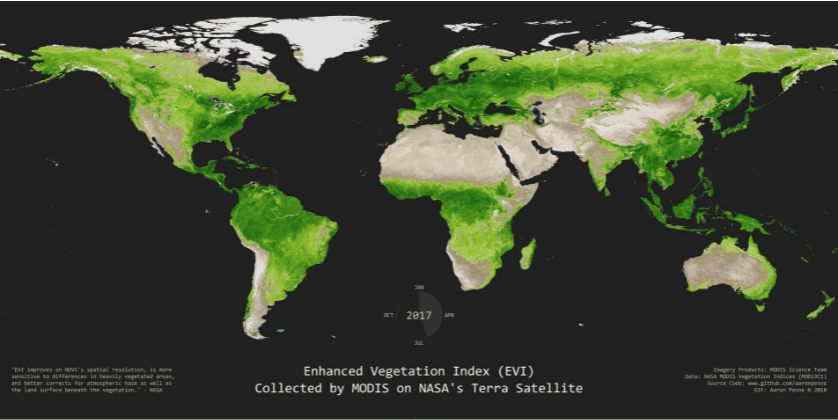
\includegraphics[width=\textwidth]{mp4/apenne_modis_ndvi.png}}{mp4/apenne_modis_ndvi.mp4}
		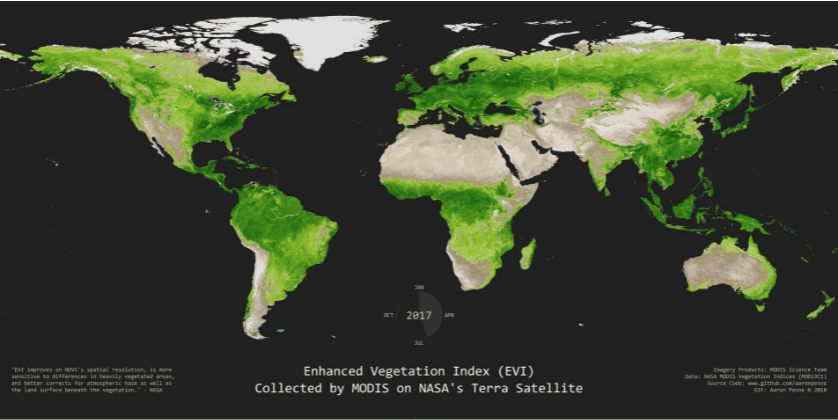
\includegraphics[width=\textwidth]{mp4/apenne_modis_ndvi.png}
		
		{\tiny visualization \href{https://github.com/aaronpenne}{Aaron Penne Github}}
		
	\end{frame}
	
	\begin{frame}{Label Data in Abundance}
		\begin{tikzpicture}
			\node{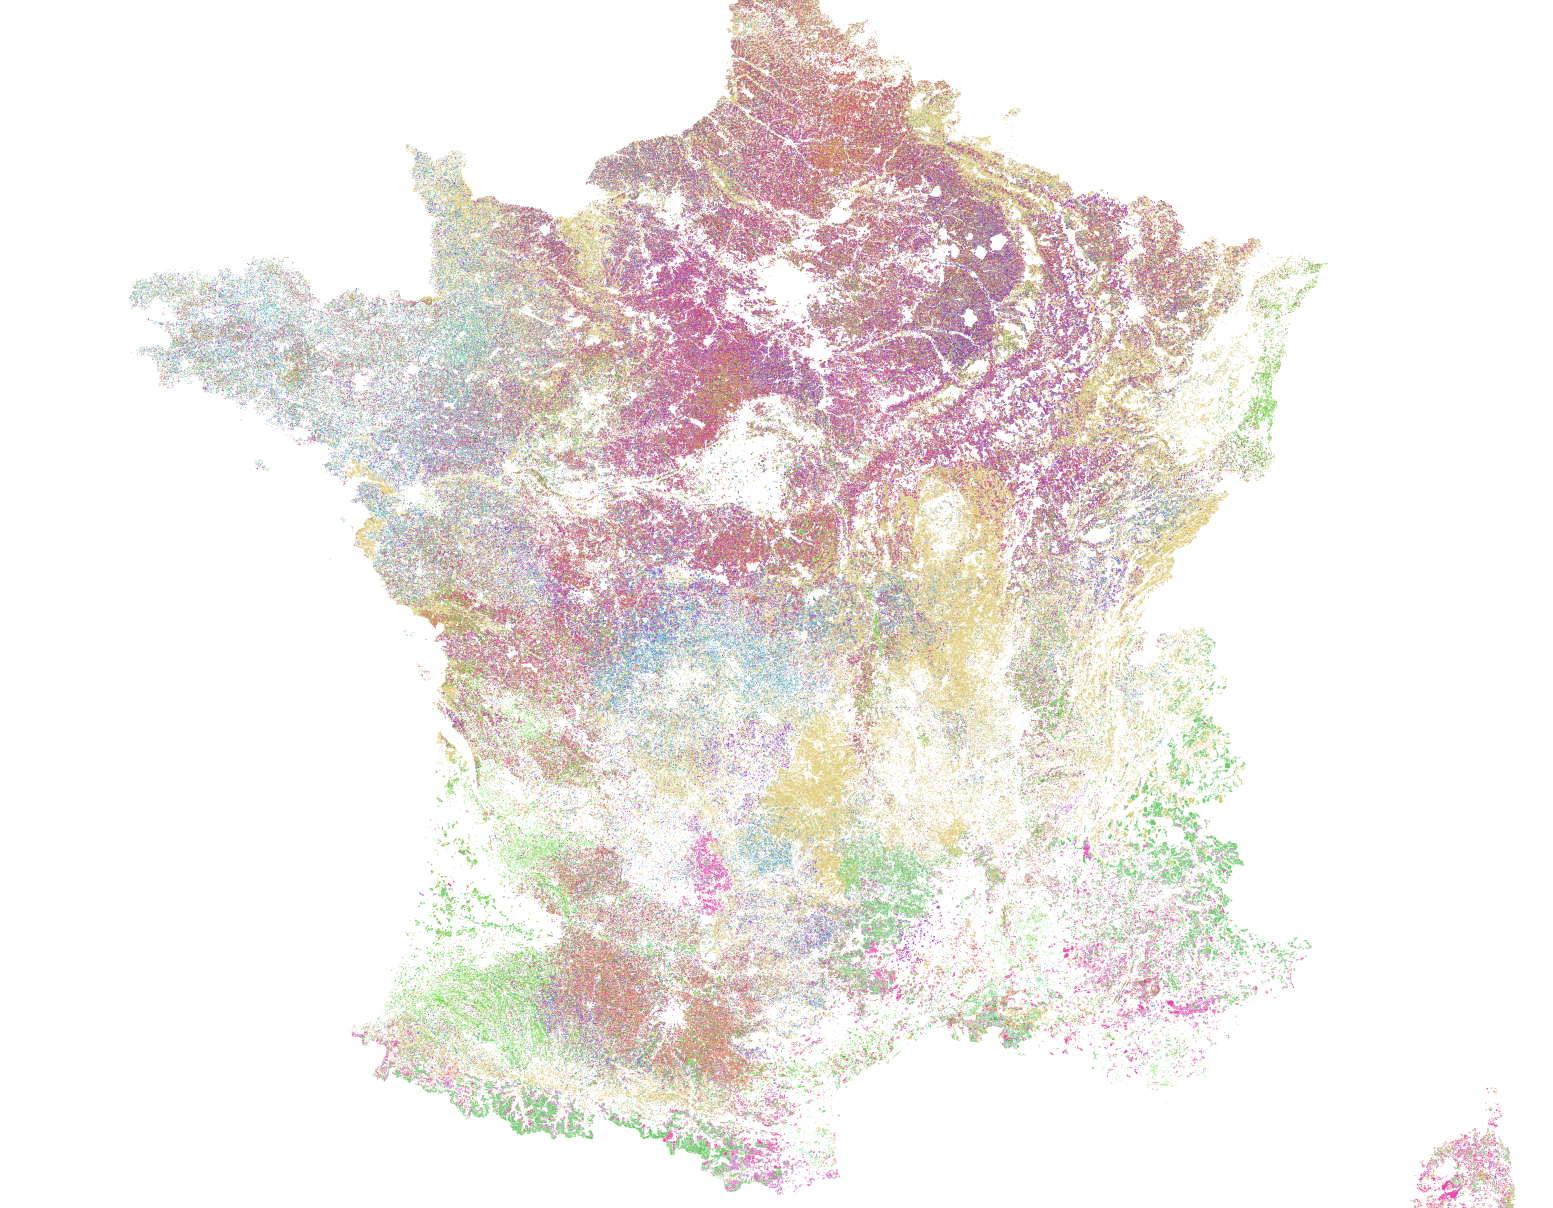
\includegraphics[width=\textwidth]{images/france_crop_distribution}};
			\visible<2>{
				\node[anchor=west, text=white, fill=rouge, text width=8cm] at (-5,-3){10 million field labels, in France each year. \\ 3 GB in labels and 2.7 TB in (Sentinel 2) satellite data};
			}
		\end{tikzpicture}
	
	\end{frame}

	\begin{frame}[plain]
		\centering
		\vfill
		
		\Large
		Problem Solved?
		
		\visible<2->{
			\vspace{2em}
			Plenty of input data!
		}
	
		\visible<3->{
			\vspace{2em}
			Plenty of labelled data!
		}

		\visible<4>{
			\vspace{2em}
			\textbf{Let's train a Deep Learning Model!}
		}
		
		\vfill
		
	\end{frame}

	\begin{frame}{The "Data Dilemma"}
		\begin{tikzpicture}
			\node(a){
				\only<1>{
					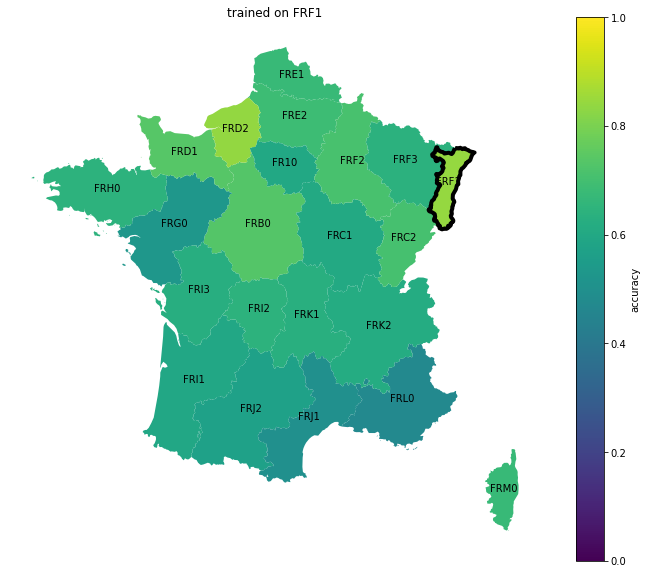
\includegraphics[width=.8\textwidth]{images/francecrops/frf1.png}
				}
%				\only<2>{
%					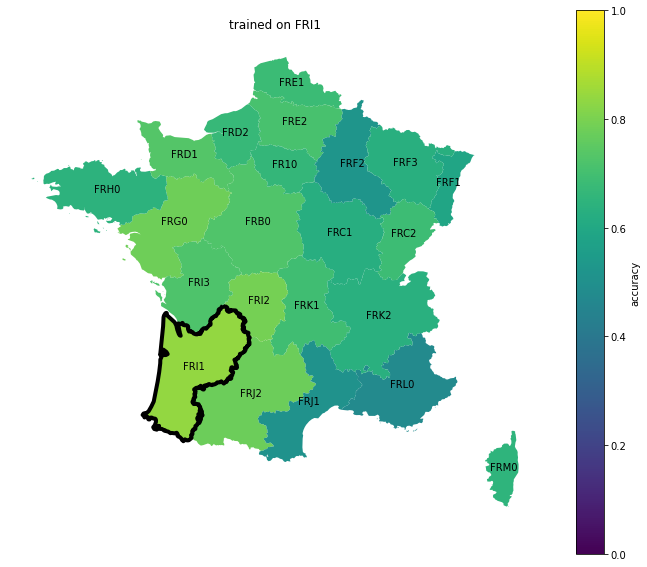
\includegraphics[width=.8\textwidth]{images/francecrops/fri1.png}
%				}
			};
			\node[left=-3em of a, text width=3cm]{training and testing on different regions};
		\end{tikzpicture}
		
		\vspace{-.5cm}
		binary "wheat" vs "other cereals" classification
		
%		\vspace{1em}
		{\tiny 
			crop type time series classification with a simple 1D-CNN and 200 samples per class	in each NUTS-2 region
		}
	\end{frame}

%
%	\begin{frame}{Training and Testing on different regions}
%		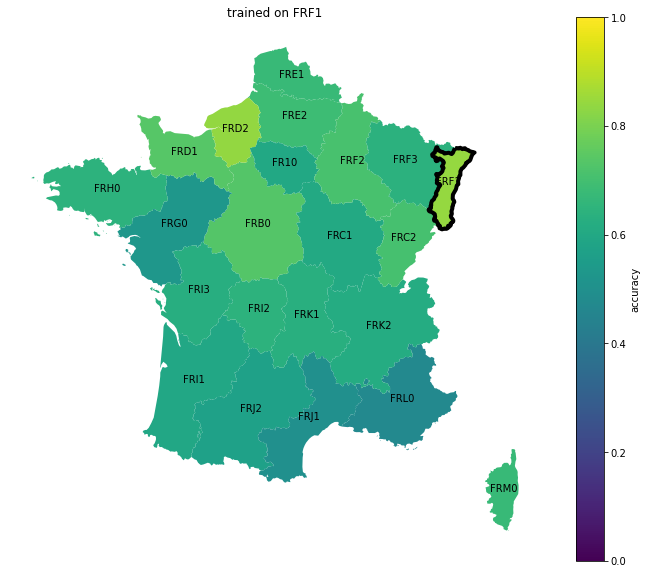
\includegraphics[width=.49\textwidth]{images/francecrops/frf1.png}
%		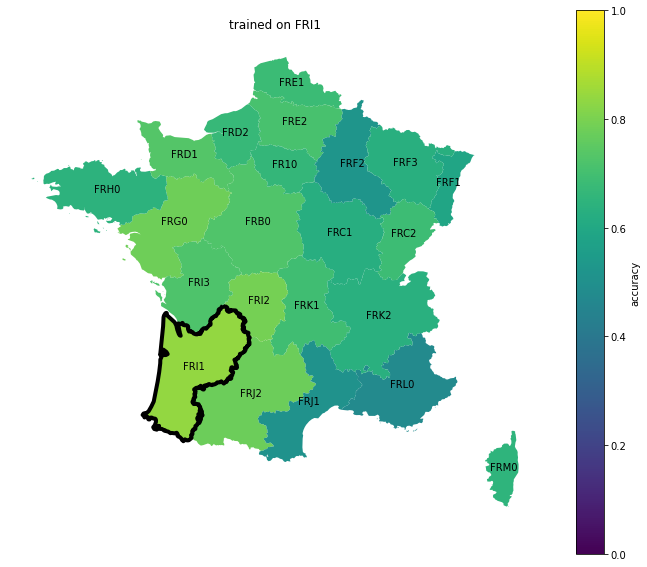
\includegraphics[width=.49\textwidth]{images/francecrops/fri1.png}
%		
%		\vspace{1em}
%		binary "wheat" vs "other cereals" classification
%		
%		\vspace{1em}
%		{\small 
%			crop type time series classification with a simple 1D-CNN and 200 samples per class	in each NUTS-2 region
%		}
%	\end{frame}
	
	\begin{frame}{Environmental Conditions}
		
				
		{
			Photosynthesis is a function of the environment.
		}
	
		\vspace{1cm}
		
		\begin{columns}[t]
			\column{.5\textwidth}
			Precipitation 2018-08
			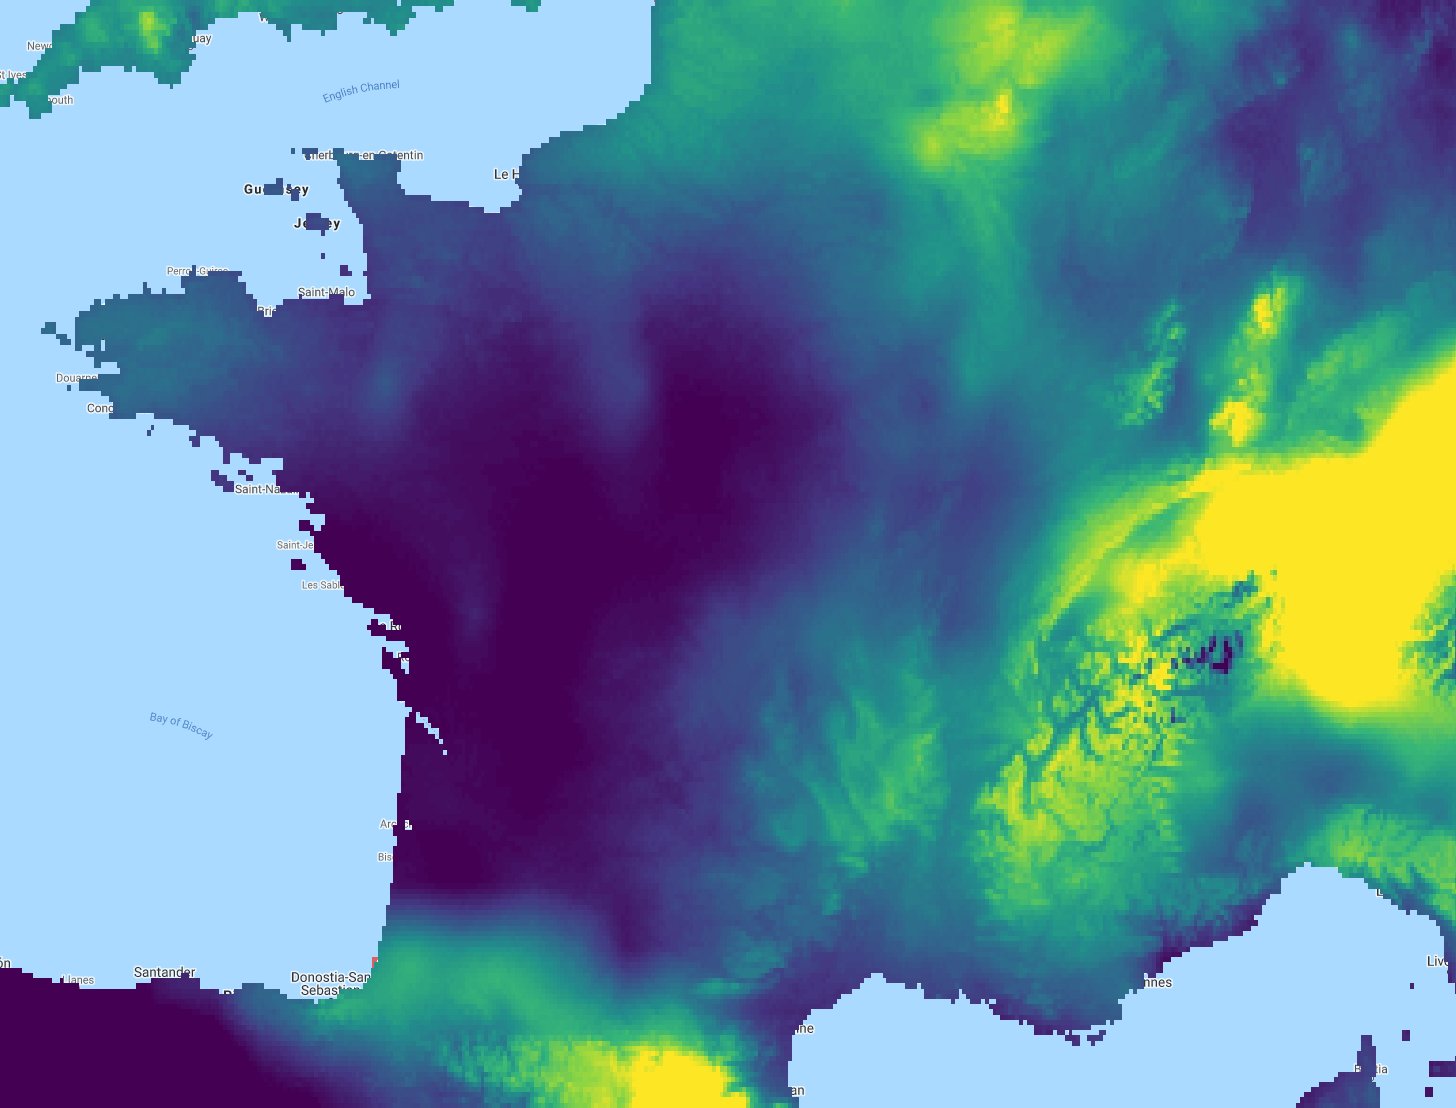
\includegraphics[width=\textwidth]{images/france_pr_201808}
			
			\column{.5\textwidth}
				Max temp (23-30°C) 2018-08
				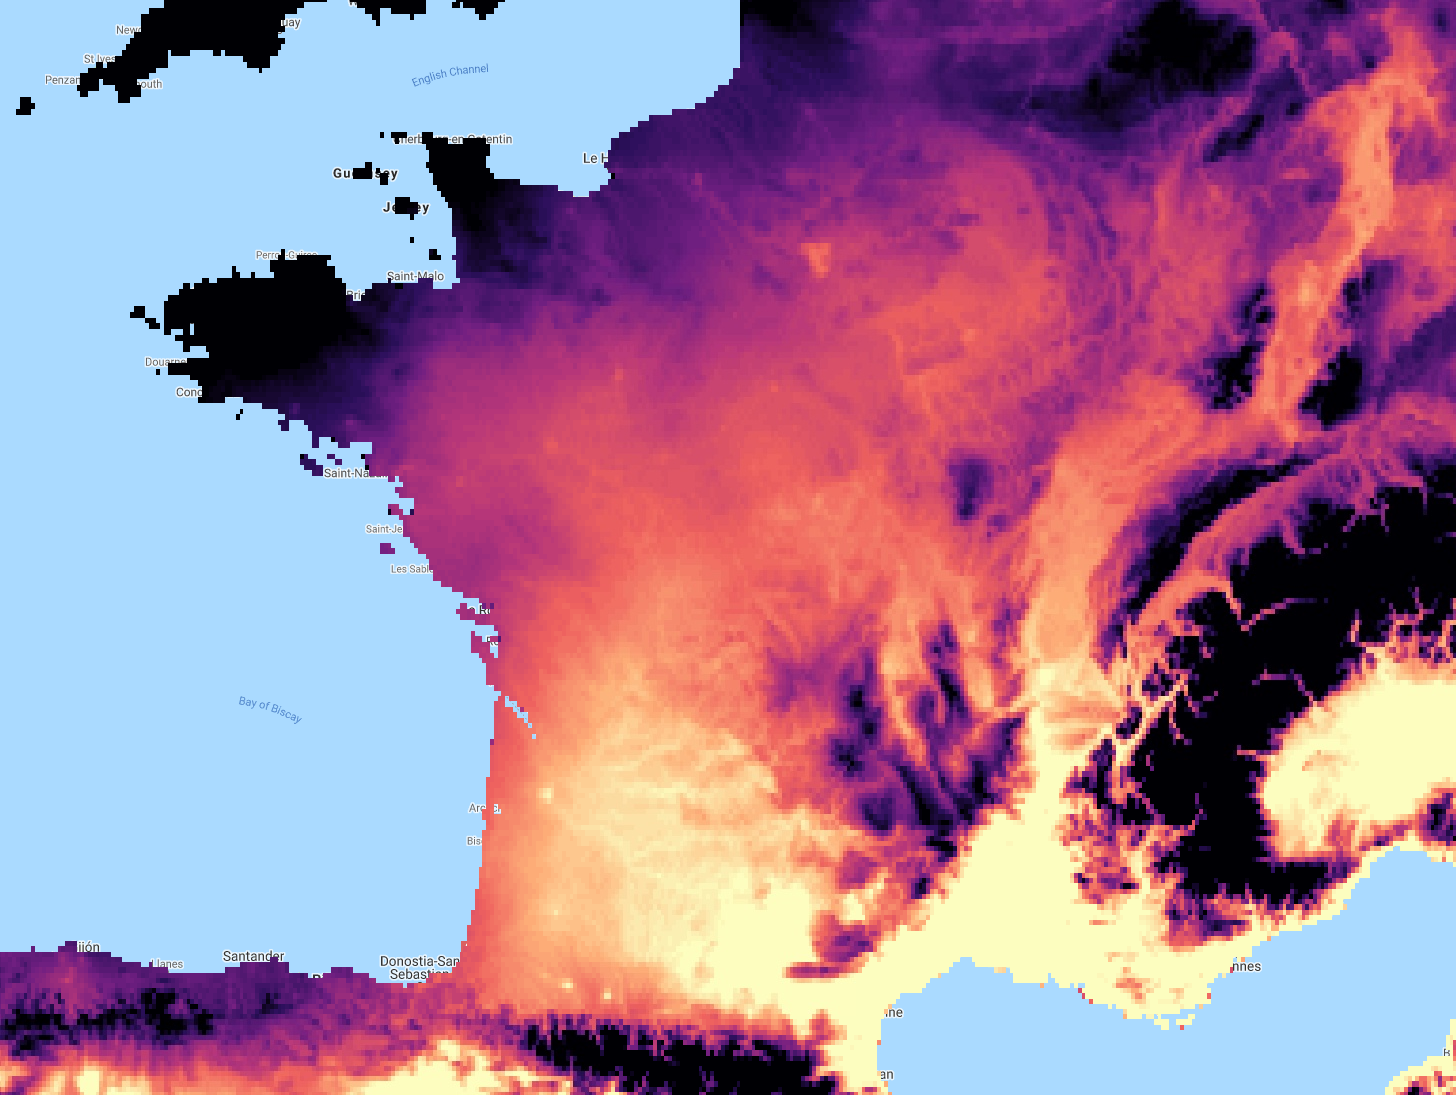
\includegraphics[width=\textwidth]{images/france_tmmx_201808}
			
		\end{columns}

	\end{frame}
	
	\begin{frame}{Apply models on regions of little data}
		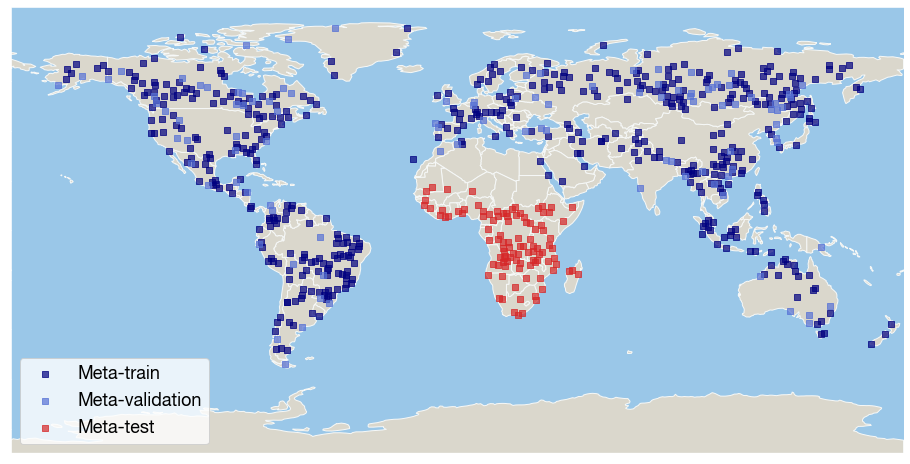
\includegraphics[width=\textwidth]{igarss2020/modis_task_map}
	\end{frame}

	
	


%	\begin{frame}[plain]
%		\centering
%		\hfill
%		\Large
%		
%		Model- and Data-Driven Approaches
%		\hfill
%	\end{frame}
%
%	\begin{frame}{Model-Driven Methods {\small (until 2017)}}
%		
%		\begin{columns}
%			\column{.5\textwidth}
%				\resizebox{\textwidth}{!}{
%					\begin{tikzpicture}
%					\node[label={above:\scriptsize growth stages of corn Mimic et al 2020}, inner sep=0](a){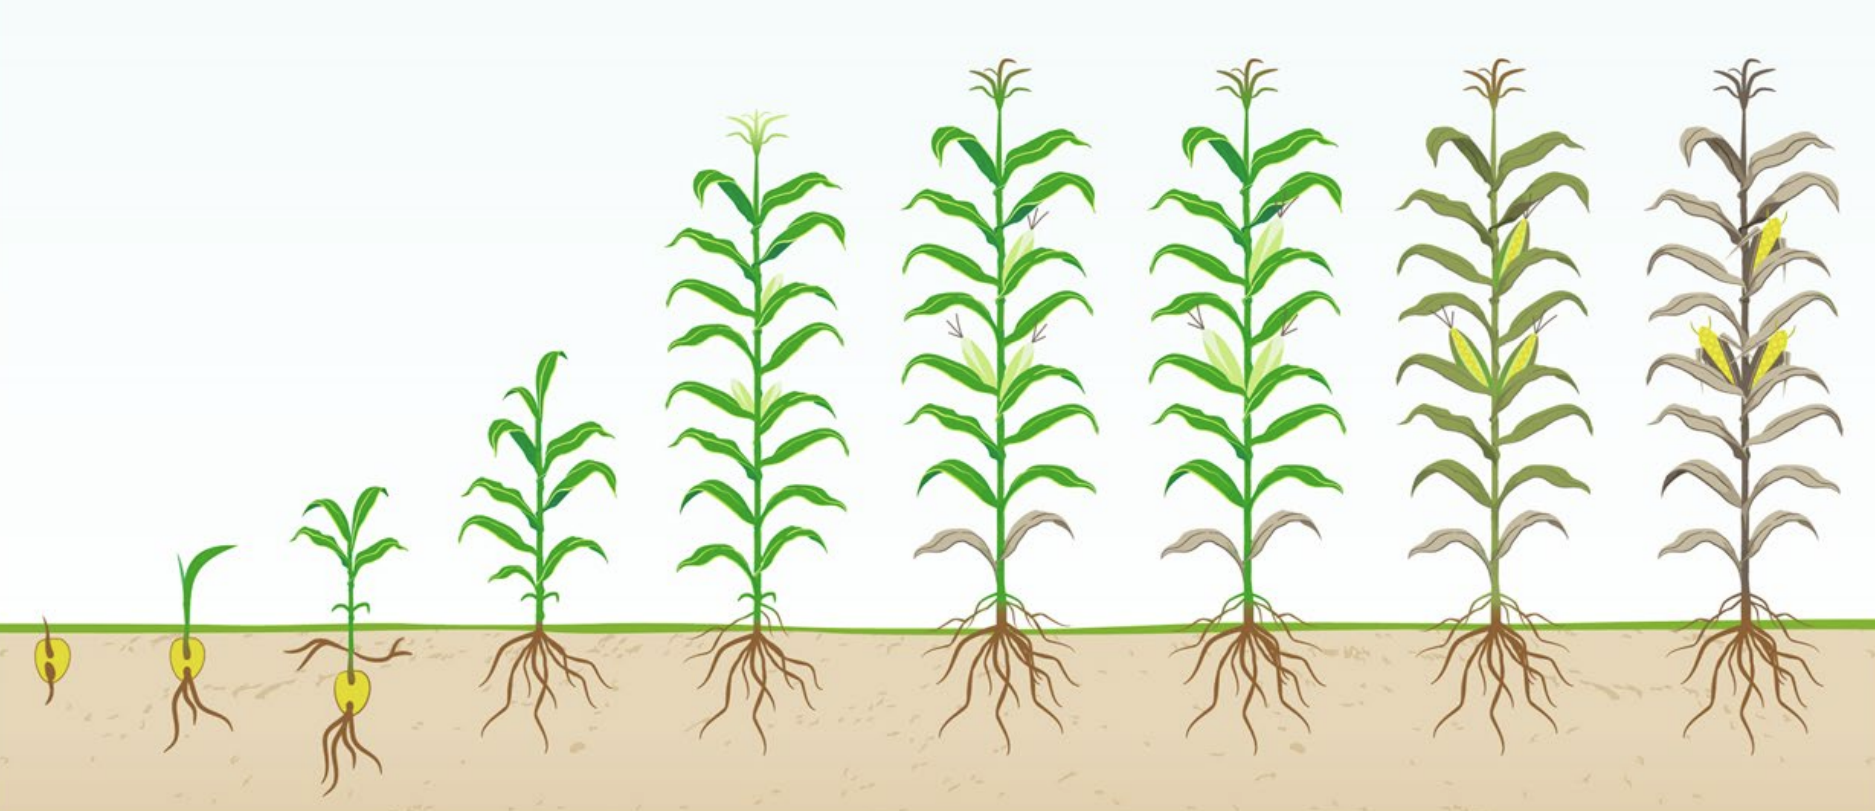
\includegraphics[width=6cm]{images/example/mimicetal2020_phenology_maize_}};
%					
%					\node[below=1em of a] (b){\includegraphics{images/example/NDVI}};
%					
%					\coordinate(left)  at ($(a.south west)+(-4.3em,0)$);
%					\coordinate(right) at ($(a.south east)+(1.1em,0)$);
%					
%					\coordinate(veannot) at ($(left)!0.22!(right)$){};
%					\coordinate(vtwoannot) at ($(left)!0.275!(right)$){};
%					\coordinate(vfiveannot) at ($(left)!0.34!(right)$){};
%					\coordinate(vtenannot) at ($(left)!0.42!(right)$){};
%					\coordinate(btnnot) at ($(left)!0.5!(right)$){};
%					\coordinate(rtwoannot) at ($(left)!0.6!(right)$){};
%					\coordinate(rthreeannot) at ($(left)!0.7!(right)$){};
%					\coordinate(rfiveannot) at ($(left)!0.8!(right)$){};
%					\coordinate(harvestannot) at ($(left)!0.9!(right)$){};
%					
%					\coordinate(ve) at      ($ (b.center)+(-4em  ,1em) $);
%					\coordinate(vtwo) at    ($ (b.center)+(-3em  ,1em) $);
%					\coordinate(vfive) at   ($ (b.center)+(-2.5em,3em) $);
%					\coordinate(vten) at    ($ (b.center)+(-2em  ,4em) $);
%					\coordinate(bt) at      ($ (b.center)+(-1.5em,4.5em) $);
%					\coordinate(rtwo) at    ($ (b.center)+(-1em  ,4.5em) $);
%					\coordinate(rthree) at  ($ (b.center)+(-0em  ,2em) $);
%					\coordinate(rfive) at   ($ (b.center)+(1.5em ,0.5em) $);
%					\coordinate(harvest) at ($ (b.center)+(3em   ,0.5em) $);
%					
%					\draw[Circle-,tumorange](veannot)      -- (ve);
%					\draw[Circle-,tumorange](vtwoannot)    -- (vtwo);
%					\draw[Circle-,tumorange](vfiveannot)   -- (vfive);
%					\draw[Circle-,tumorange](vtenannot)    -- (vten);
%					\draw[Circle-,tumorange](btnnot)       -- (bt);
%					\draw[Circle-,tumorange](rtwoannot)    -- (rtwo);
%					\draw[Circle-,tumorange](rthreeannot)  -- (rthree);
%					\draw[Circle-,tumorange](rfiveannot)   -- (rfive);
%					\draw[Circle-,tumorange](harvestannot) -- (harvest);
%					\end{tikzpicture}
%				}
%			\column{.5\textwidth}
%				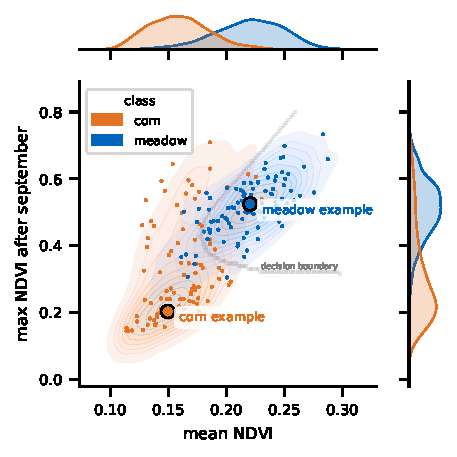
\includegraphics[width=\textwidth]{images/example/jointplot}
%			
%		\end{columns}
%	
%		\begin{tikzpicture}
%			\tikzstyle{process} = [draw, rounded corners]
%			\node(x){input $\mathbf{X}$};
%			\node[process, right=of x](f){feature definition};
%			\node[process, right=of f](c){classification};
%			\node[right=of c](y){label $y$};
%			\draw[-Stealth](x) -- (f);
%			\draw[-Stealth](f) -- (c);
%			\draw[-Stealth](c) -- (y);
%			\node[below=0cm of f, font=\scriptsize](a){mean NDVI};
%			\node[below=0cm of a, font=\scriptsize](b){max NDVI after Sept};
%			
%			\node[below=0cm of c, font=\scriptsize](a){e.g., SVM, RF};
%		\end{tikzpicture}
%		
%		\vspace{1em}
%		\visible<2>{
%			\centering\textbf{What are the best features?}
%		}
%		
%	\end{frame}

	
	\newcommand{\nn}{
		\tikzstyle{proba} = [circle, draw=white, inner sep=2.5pt, fill=rouge]
		\begin{tikzpicture}[scale=0.5, rotate=0, baseline=-.25em, minimum width=0cm, minimum height=0cm]
		\node[proba](a0) at (0,-1){};
		\node[proba](a1) at (0,0){};
		\node[proba](a2) at (0,1){};
		
		\node[proba](b0) at (1,-0.5){};
		\node[proba](b1) at (1,0.5){};
		
		\draw[-] (a0) -- (b0);
		\draw[-] (a1) -- (b0);
		\draw[-] (a2) -- (b0);
		
		\draw[-] (a0) -- (b1);
		\draw[-] (a1) -- (b1);
		\draw[-] (a2) -- (b1);
		
		%	\node[fit=(a0)(a2)(b1)](node name){};
		
		\end{tikzpicture}
	}

	\newcommand{\featurelearningtikz}{
		\begin{tikzpicture}
			\tikzstyle{process} = [draw, rounded corners]
			\node(x){input $\mathbf{X}$};
			\node[process, right=of x](f){feature learning $f_\mathbf{\theta}$ \nn};
			\node[right=of f](y){label $y$};
			\draw[-Stealth](x) -- (f);
			\draw[-Stealth](f) -- (y);
		\end{tikzpicture}
	}
%
%	\begin{frame}[t]{Data-Driven Methods}
%		
%		
%		\centering
%		\featurelearningtikz
%		
%		\vspace{1em}
%		
%		\raggedright
%		
%		\resizebox{\textwidth}{!}{
%			\colorlet{tumgray}{gray}
\tikzstyle{annotation} = [font=\small, text width=3.5cm]
\tikzstyle{node} = [circle, draw, font=\small]
\tikzstyle{edge} = [-stealth, tumgray]
\tikzstyle{operation} = [font=\scriptsize, fill=white, text=black]
\tikzstyle{normal} = [font=\scriptsize, text=tumblue]
\begin{tikzpicture}[node distance=0]



\node(a){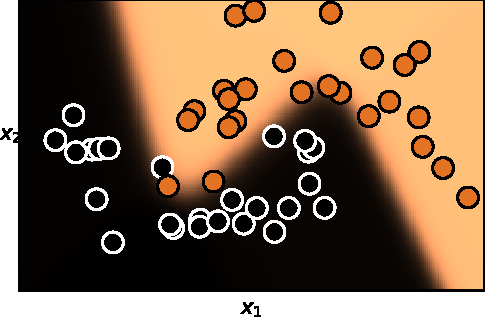
\includegraphics[width=3cm]{nn/x.pdf}};
\node[right=of a](b){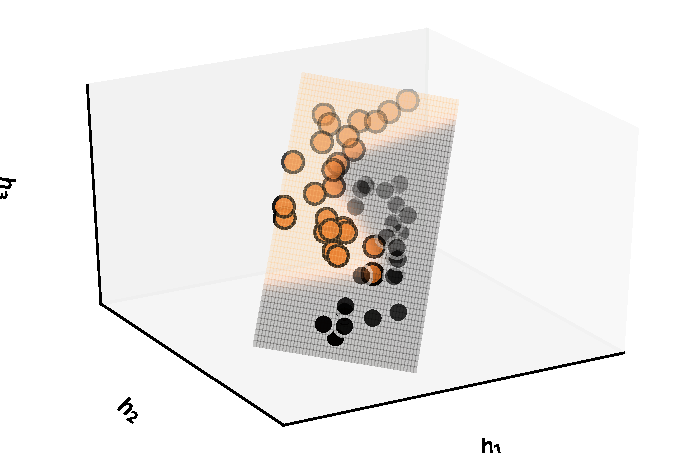
\includegraphics[width=4.5cm]{nn/h.pdf}};
\node[right=of b](c){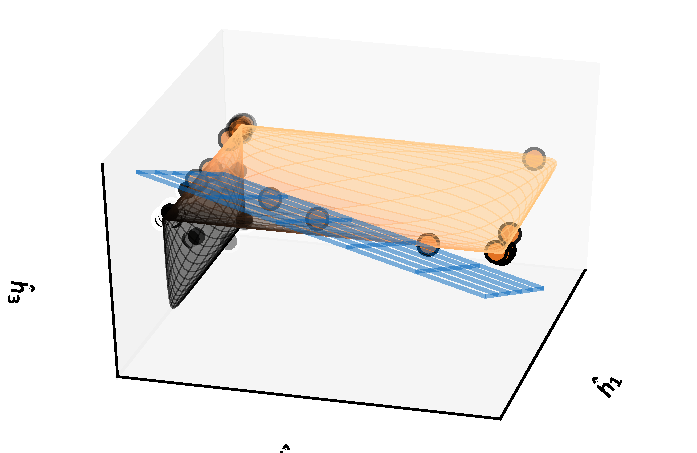
\includegraphics[width=4.5cm]{nn/h2.pdf}};
\node[right=1em of c](d){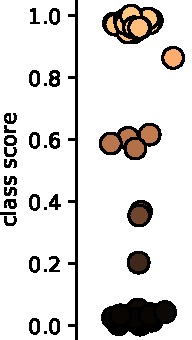
\includegraphics[width=1.2cm]{nn/y.pdf}};

\coordinate(annotations) at (0,-3);
\node[annotation] at (a |- annotations){(a) Input space \\ $\mathbf{x} = (x_1, x_2)$};
\node[annotation] at (b |- annotations){(b) linear projection $\mathbf{w}_1^T\mathbf{x}$ into $\mathbb{R}^3$};
\node[annotation, xshift=-2em] at (c |- annotations){(c) non-linear distortion with $\tanh(\mathbf{w}_1^T\mathbf{x})$};
\node[annotation] at (d |- annotations){(d) Output class probabilities $y \in [0,1]$};

\coordinate(network) at (0,3);
\coordinate(networklone) at (a |- network);
\coordinate(networkltwo) at (b |- network);
\coordinate(networklthree) at (c |- network);
\coordinate(networklast) at (d |- network);

\node[node, above=of networklone](xone){$x_1$};
\node[node, below=of networklone](xtwo){$x_2$};
\begin{scope}[node distance=1.3em]
\node[node, above=of networkltwo](hone){$h_1$};
\node[node] at (networkltwo)(htwo){$h_2$};
\node[node, below=of networkltwo](hthree){$h_3$};
\end{scope}

\begin{scope}[node distance=1.3em]
\node[node, above=of networklthree](hhone){$\hat{h}_1$};
\node[node] at (networklthree)(hhtwo){$\hat{h}_2$};
\node[node, below=of networklthree](hhthree){$\hat{h}_3$};
\end{scope}

%			\node[node] at (networklthree){a};
\node[node](y) at (networklast){$y$};

\draw[edge] (xone) -- (hone);
\draw[edge] (xone) -- (htwo);
\draw[edge] (xone) -- (hthree);
\node[operation] at ($(networklone)!0.5!(networkltwo)$) {$\mathbf{W}_1$};

\draw[edge] (xtwo) -- (hone);
\draw[edge] (xtwo) -- (htwo);
\draw[edge] (xtwo) -- (hthree);

\draw[edge] (hone) -- node[midway]{} (hhone);
\draw[edge] (htwo) -- node[midway, operation]{$\tanh$} (hhtwo);
\draw[edge] (hthree) -- node[midway]{} (hhthree);

\draw[edge] (hhthree) -- node[near start, below, normal, name=lastweight]{$w_{2,3}$} (y);
\draw[edge] (hhone) -- node[near start, below, normal]{$w_{2,1}$} (y);
\draw[edge] (hhtwo) -- node[near start, below, normal]{$w_{2,2}$} node[near end, operation]{$\Sigma \circ \sigma$} (y);

\draw[-stealth, tumblue] (lastweight) to[bend left] node[near start, yshift=1em, right, font=\tiny, text width=3.5cm]{$\mathbf{w}_2 = (w_{2,1},w_{2,2},w_{2,3})$ defines the normal of the decision plane} ++(-1,-2);

%\draw[decorate, decoration = {brace}] ($(networklone)+(0,4em)$) -- node[midway, above, font=\small]{feature extraction} ($(networklthree)+(0,4em)$);
%\draw[decorate, decoration = {brace}] ($(networklthree)+(0,4em)$) -- node[midway, above, font=\small]{classification} ($(networklast)+(0,4em)$);

\end{tikzpicture}
%		}
%	
%		\vspace{1em}
%		\visible<2>{
%			\centering\textbf{What are the best DL models?}
%		}
%	\end{frame}
%
%	\begin{frame}[t]{Data-Driven Methods}
%		\centering
%		\featurelearningtikz
%		
%		\raggedright
%		\hspace{-1em} Search for suitable data-specific architecture
%			
%			{ 
%%				\begin{columns}[t]
%					
%%					\column{.5\textwidth}
%					
%					\vspace{1em}
%					
%					In general
%						\begin{itemize}
%							\item CNNs for images (e.g. ResNet50)
%							\item Transformers for language (e.g. Bert)
%							\item RNNs for state-memory problems (e.g. hydrological modeling).
%						\end{itemize}
%%					\column{.5\textwidth}
%					
%%					For crop type mapping
%%					\begin{itemize}
%%						\item CNNs 
%%						\item RNNs 
%%						\item Transformers
%%					\end{itemize}
%				
%%				\end{columns}
%			}
%		\pause
%		\vspace{2em}
%			\raggedright
%			{Data-driven deep learning models are very plastic and (blindly) learn to approximate target data.}\\
%			\pause
%			\vspace{1em}
%			We need to \textbf{think carefully} how \textbf{we sample} and \textbf{select data}. 
%			
%	\end{frame}

	\begin{frame}[plain]
		\centering
		\hfill
		\Large
		
		How do we generate data?
%		What assumptions do we take in \\ Machine Learning?
		
		
		\hfill
\end{frame}

	\newcommand{\iidsim}{\mathrel{\overset{\makebox[0pt]{\mbox{\normalfont\tiny\sffamily i.i.d}}}{\sim}}}
	\begin{frame}[t]{Data Generation Model}
		\centering
%		
%		\featurelearningtikz
%		
%		\vspace{1em}
		
		\begin{tikzpicture}
			\node[label={[name=domainlabel]domain}](domain){$\mathcal{D} = \{\mathcal{X}, P(\mathcal{X})\}$};
			\visible<3->{
				\node[label={[name=tasklabel]task}, right=of domain](task){$\mathcal{T} = \{\mathcal{Y}, f(\cdot)\}$};
			}
			
			\visible<2->{
				\node[below=of domain](xsample){$\mathbf{X} \sim P(\mathcal{X})$};
				\draw[-Stealth] (domain) -- (xsample);
			}
			
			\visible<4->{
				\node[below=of task](ysample){$y = f(\mathbf{X})$};
				\draw[-Stealth] (xsample) -- node[midway, above, font=\tiny, name=label]{predictive function f} (ysample);
			}
			\visible<5->{
				\node[fit=(domain)(xsample)(task)(ysample)(domainlabel)(tasklabel), draw, rounded corners, label={[name=dgm, font=\small]below:joint data distribution $P(\mathcal{X} \times \mathcal{Y})$}](box) {};
	%			\node[right=of box, font]{Data Generation Model};
			}
			\visible<6->{
			\node[below=3em of label](datasampling){Dataset: $\{(\mathbf{X}_i,y_i)\}_{i=1}^N \iidsim P(\mathcal{X} \times \mathcal{Y})$};
			}
		
			\visible<7->{
				\node[below=1em of datasampling](model){\featurelearningtikz};
			}
		
		\end{tikzpicture}
		\vfill\tiny
		\citeapa{Pan, S. J., \& Yang, Q. (2009). A survey on transfer learning. IEEE Transactions on knowledge and data engineering, 22(10), 1345-1359.}
		\citeapa{Qiang Yang; Yu Zhang, Wenyuan Dai; Sinno Jialin Pan (Editors) (2020). Transfer learning. Cambridge University Press. DOI 9781139061773}
		\citeapa{Shai Ben-David and Shai Shalev-Shwartz (2014). Understanding Machine Learning: From Theory to Algorithms}
	\end{frame}

%	\begin{frame}[plain]
%		\centering
%		\hfill
%		\Large
%		
%		Our central Assumption in Machine Learning
%		%		What assumptions do we take in \\ Machine Learning?
%		
%		
%		\hfill
%	\end{frame}
%	
%	\begin{frame}
%		\frametitle{I.I.D assumption}
%		
%		we use a dataset $\{(\mathbf{X}_i,y_i)\}_{i=1}^N \iidsim P(\mathcal{X} \times \mathcal{Y})$ of \textbf{independently} and and \textbf{identically} distributed (i.i.d) samples.
%		\vspace{1em}
%		
%%		\pause
%		we need \textbf{independence} for the factorization in max likelihood.
%		\begin{align*}
%		\theta^\ast &= \arg\max_\theta \prod_{i} p(y_i \vert \mathbf{X}_i)  \\
%		&= \arg\min_\theta \sum_{i} -y_i \log f_\theta(\mathbf{X}_i)
%		\end{align*}
%		
%		\pause
%		we assume an \textbf{identical} (joint) \textbf{distribution} $P(\mathcal{X} \times \mathcal{Y})$ throughout the entire data generation { \scriptsize (and particularly between training and test time) }
%		\begin{align}
%		X_i,y_i \iidsim P(\mathcal{X} \times \mathcal{Y})
%		\end{align}
%		which implies identical domains $\mathcal{D} = \{\mathcal{X}, P(\mathcal{X})\}$ and tasks $\mathcal{T} = \{\mathcal{Y}, f(\cdot)\}$ during training and test time.
%		
%	\end{frame}

	\begin{frame}{In- and Out-of-Dist. Generalization}
		
		The I.I.D assumption is usually enforced via random splitting a single dataset $D$ into training and testing partitions
		
		\vspace{2em}
		
		\begin{tikzpicture}
			\node(ds) at (0,0){$D \iidsim P(\mathcal{X} \times \mathcal{Y})$};
			\node at (-1,-1)(dstrain){$D_\text{train}$};
			\node at (1,-1)(dstest){$D_\text{test}$};
			
			\draw[-Stealth](ds) --node[midway, left=1em, font=\tiny, name=labelsplit]{random split} (dstrain);
			\draw[-Stealth](ds) -- (dstest);
			
			\node[draw, rounded corners, fit=(ds)(dstrain)(dstest)(labelsplit), label={above: I.I.D Machine Learning}](b1){};
			
			\node[below=of dstrain, label={[font=\tiny]below:train model}] (weights) {$f_\theta$};
			\draw[-Stealth] (dstrain) -- (weights);


			\node[below=of dstest] (testloss) {$\mathcal{L}_\text{in}$};
			\draw[-Stealth] (dstest) -- (testloss);
			\draw[-Stealth] (weights) -- node[midway,above,font=\tiny]{compare with $f(\cdot)$} (testloss);
			
			\node[below=0em of testloss, text width=2cm, font=\scriptsize](tllabel){"in-domain" or "in-distribution" generalization};
			
			\visible<2->{
				\node[right=5em of ds](Q){$\mathbf{X},y \sim Q(\mathcal{X} \times \mathcal{Y})$};
				
				\node[below=0em of Q](domain){$\mathcal{D}_Q = \{\mathcal{X}, P_Q(\mathcal{X})\}$};
				\node[below=-.5em of domain](task){$\mathcal{T}_Q = \{\mathcal{Y}, f_Q(\cdot)\}$};
				
				\node[rounded corners, fit=(Q)(domain)(task), label={above: Data of another distribution\phantom{g}}](b2){};
				
				\node[right=8em of testloss] (oodloss) {$\mathcal{L}_\text{out}$};
				\node[below=0em of oodloss, text width=3cm, font=\scriptsize](oodlabel){"out-of-domain" or \\ "out-of-distribution" \\ generalization};
				
				\draw[-Stealth] (testloss) -- node[midway,above,font=\tiny]{compare with $f_Q(\cdot)$} (oodloss);
				\draw[-Stealth] (task) -- (oodloss);
			}
		
			\visible<3->{
				\node[fill=white, fill opacity=0.5, text opacity=1] at (b1) {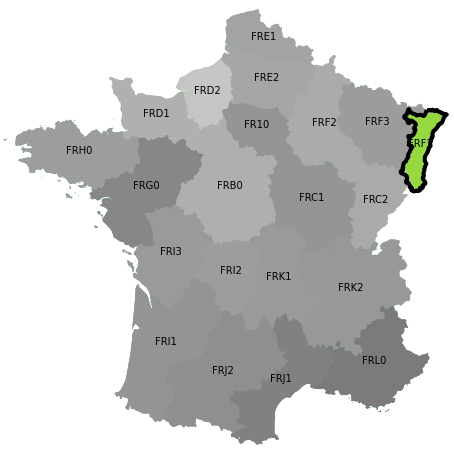
\includegraphics[width=4cm]{images/francecrops/frf1_train_highlighted}};
				\node[fill=white, fill opacity=0.5, text opacity=1] at (b2) {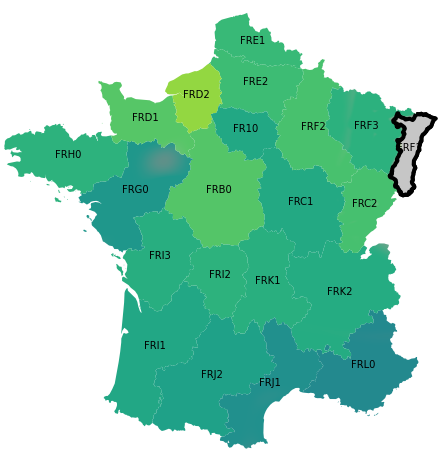
\includegraphics[width=4cm]{images/francecrops/frf1_test_highlighted}};
			}
		\end{tikzpicture}
	\end{frame}


%	\begin{frame}{Train/Test Dists are usually not identical}
%		
%		Examples
%		\begin{columns}[t]
%			\column{.5\textwidth}
%			
%			gender classification \\
%			{\scriptsize (Buolamwini \& Gebru, 2016)}
%			
%			\vspace{1em}
%			
%			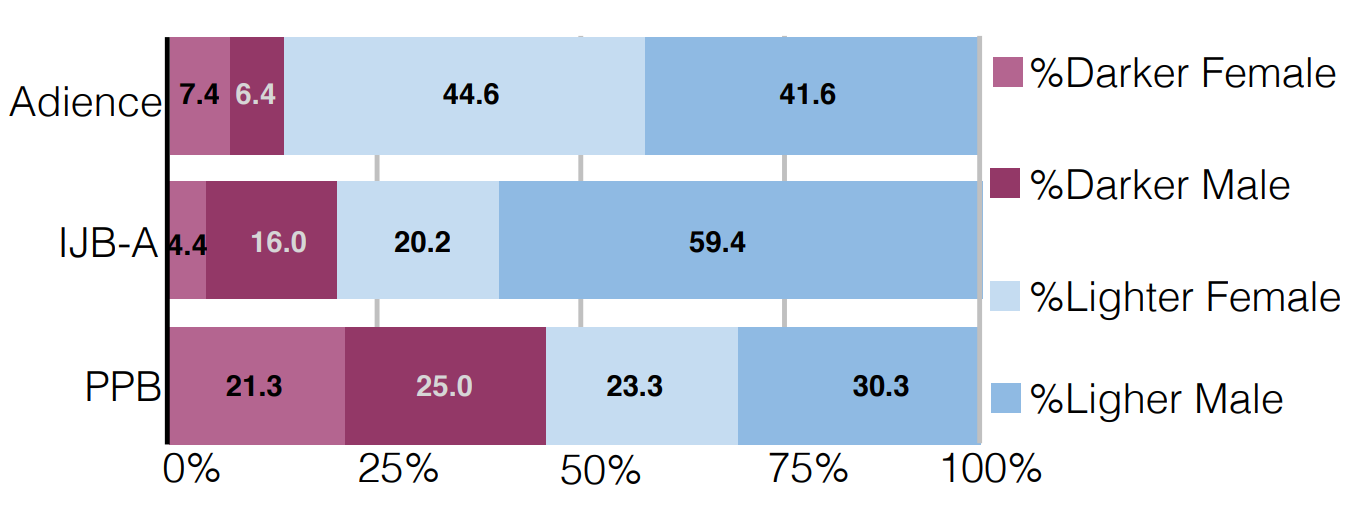
\includegraphics[width=\textwidth]{images/BoulamwiniGebru2016}
%			
%			\vspace{1em}
%			
%			CV classifiers performed
%			\begin{itemize}
%				\item worst for darker females
%				\item best for lighter males
%			\end{itemize}
%			
%			\column{.5\textwidth}
%			
%			large language models
%			
%			\begin{itemize}
%				\item Trained on massive text datasets on the internet (e.g. Reddit, News, Blogs).
%				\item deployed in everyday situations (e.g. chat bots,  drafting blog posts).
%			\end{itemize}
%			
%			Strereotyp-bias is encoded via the training dataset and can be quantified {\scriptsize (Nadeem et al., 2020)}
%			
%		\end{columns}
%		
%		\vfill
%		
%		\citeapa{Buolamwini, J., \& Gebru, T. (2018, January). Gender shades: Intersectional accuracy disparities in commercial gender classification. In Conference on fairness, accountability and transparency (pp. 77-91). PMLR.}
%		
%		\citeapa{Nadeem, M., Bethke, A., \& Reddy, S. (2020). Stereoset: Measuring stereotypical bias in pretrained language models. arXiv preprint arXiv:2004.09456.}
%	\end{frame}

%	\begin{frame}{Measuring OOD Generalization}
%		\begin{tikzpicture}
%		\node(ds) at (0,0){$D \iidsim P(\mathcal{X} \times \mathcal{Y})$};
%		\node at (-1,-1)(dstrain){$D_\text{train}$};
%		\node at (1,-1)(dstest){$D_\text{test}$};
%		
%		\draw[-Stealth](ds) --node[midway, left=1em, font=\tiny, name=labelsplit]{random split} (dstrain);
%		\draw[-Stealth](ds) -- (dstest);
%		
%		\node[draw, rounded corners, fit=(ds)(dstrain)(dstest)(labelsplit), label={above: Source Task/Domain\phantom{g}}]{};
%		
%		\node[below=of dstrain, label={[font=\tiny]left:train model}] (weights) {$f_\theta$};
%		\draw[-Stealth] (dstrain) -- (weights);
%		
%		\node[below=of dstest] (testloss) {$\mathcal{L}_\text{in}$};
%		\draw[-Stealth] (dstest) -- (testloss);
%		\draw[-Stealth] (weights) -- node[midway,above,font=\tiny]{compare with $f(\cdot)$} (testloss);
%		
%		\node[below=0em of testloss, text width=2cm, font=\scriptsize](tllabel){"in-domain" or "in-distribution" generalization};
%		
%		\begin{scope}[xshift=5cm]
%			\node(Q) at (0,0){$D \iidsim Q(\mathcal{X} \times \mathcal{Y})$};
%			\node at (-1,-1)(dsqtrain){$D_\text{train}$};
%			\node at (1,-1)(dsqtest){$D_\text{test}$};
%		\end{scope}
%		
%		\draw[-Stealth](Q) --node[midway, left=0.5em, font=\tiny, name=labelqsplit]{random split} (dsqtrain);
%		\draw[-Stealth](Q) -- (dsqtest);
%		
%		\node[draw, rounded corners, fit=(Q)(dsqtrain)(dsqtest)(labelqsplit), label={above: Target Task/Domain}]{};
%		
%		\node[below=of dsqtest] (oodloss) {$\mathcal{L}_\text{out}$};
%		\node[below=0em of oodloss, text width=3cm, font=\scriptsize](oodlabel){"out-of-domain" or \\ "out-of-distribution" \\ generalization};
%		
%		\draw[-Stealth] (testloss) -- node[midway,above,font=\tiny]{compare with $f_Q(\cdot)$} (oodloss);
%		\draw[-Stealth] (dsqtest) -- (oodloss);
%		
%		\end{tikzpicture}
%	\end{frame}

%	\begin{frame}{Global Distribution Shift}
%		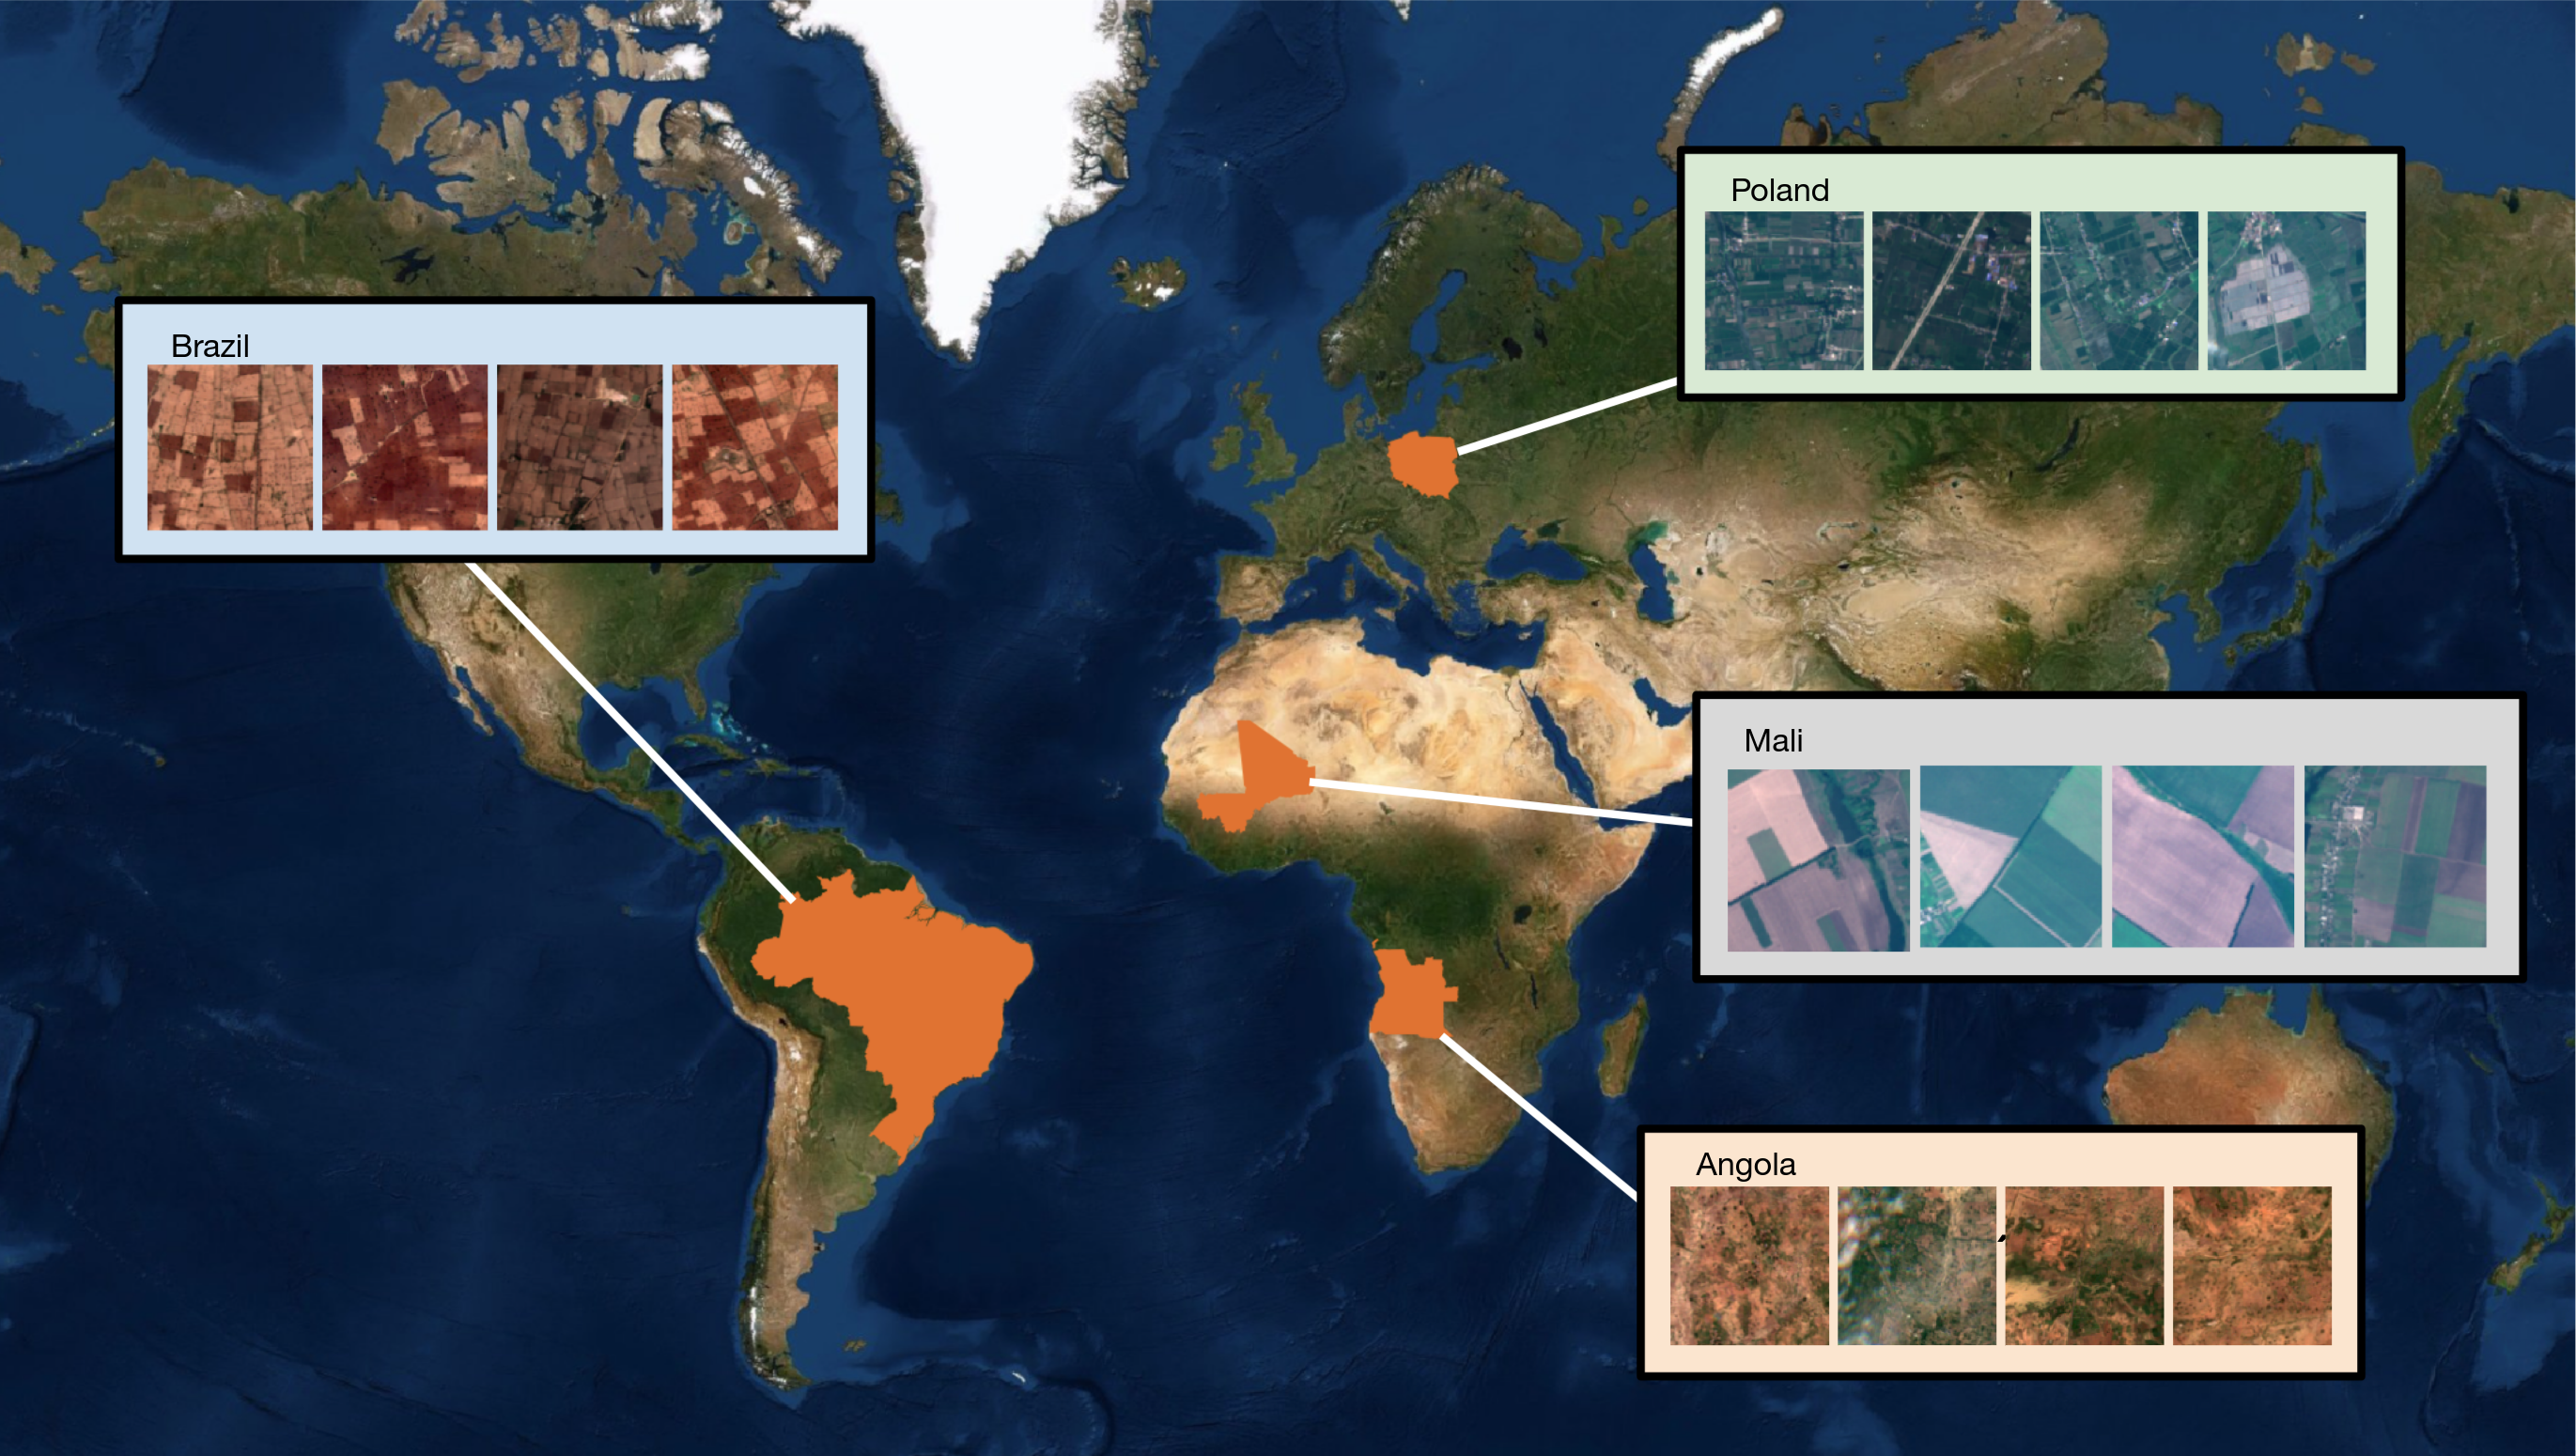
\includegraphics[width=\textwidth]{images/countries_globe}
%		
%		\vspace{0.5em}
%		
%		\scriptsize
%		Figure from
%		
%		\citeapa{Rußwurm, M., Wang, S., Körner, M., \& Lobell, D. (2020). Meta-learning for few-shot land cover classification. In Proceedings of the ieee/cvf conference on computer vision and pattern recognition workshops (pp. 200-201).}
%		
%		\scriptsize
%		Data from
%		
%		\citeapa{Schmitt, M., Hughes, L. H., Qiu, C., \& Zhu, X. X. (2019). SEN12MS--A Curated Dataset of Georeferenced Multi-Spectral Sentinel-1/2 Imagery for Deep Learning and Data Fusion. arXiv preprint arXiv:1906.07789.}
%	\end{frame}
%
%	\begin{frame}
%		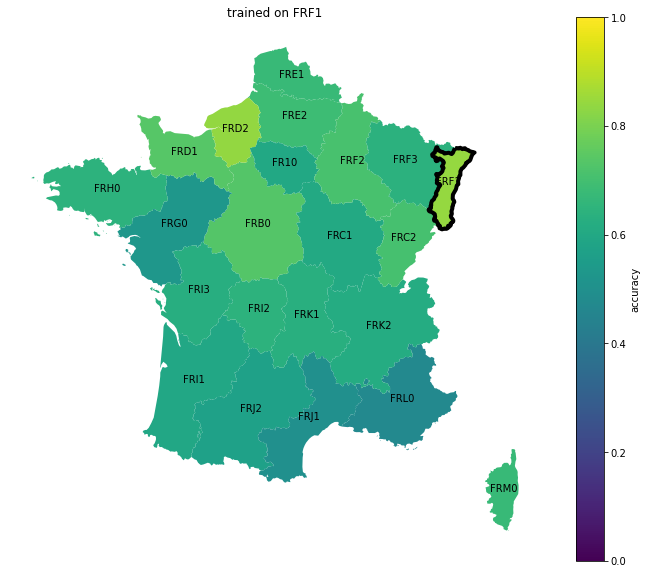
\includegraphics[width=.8\textwidth]{images/francecrops/frf1.png}
%	\end{frame}
	
	%	\begin{frame}{Domain and Task}
	%		\begin{tikzpicture}
	%		\node[label=domain](domain){$\mathcal{D} = \{\mathcal{X}, P(\mathcal{X})\}$};
	%		\node[label=task, right=of domain](task){$\mathcal{T} = \{\mathcal{Y}, f(\cdot)\}$};
	%		\end{tikzpicture}
	%		\vfill\tiny
	%		\citeapa{Pan, S. J., \& Yang, Q. (2009). A survey on transfer learning. IEEE Transactions on knowledge and data engineering, 22(10), 1345-1359.}
	%		¨
	%	\end{frame}
	
%	\begin{frame}{Global Distribution Shift}
%		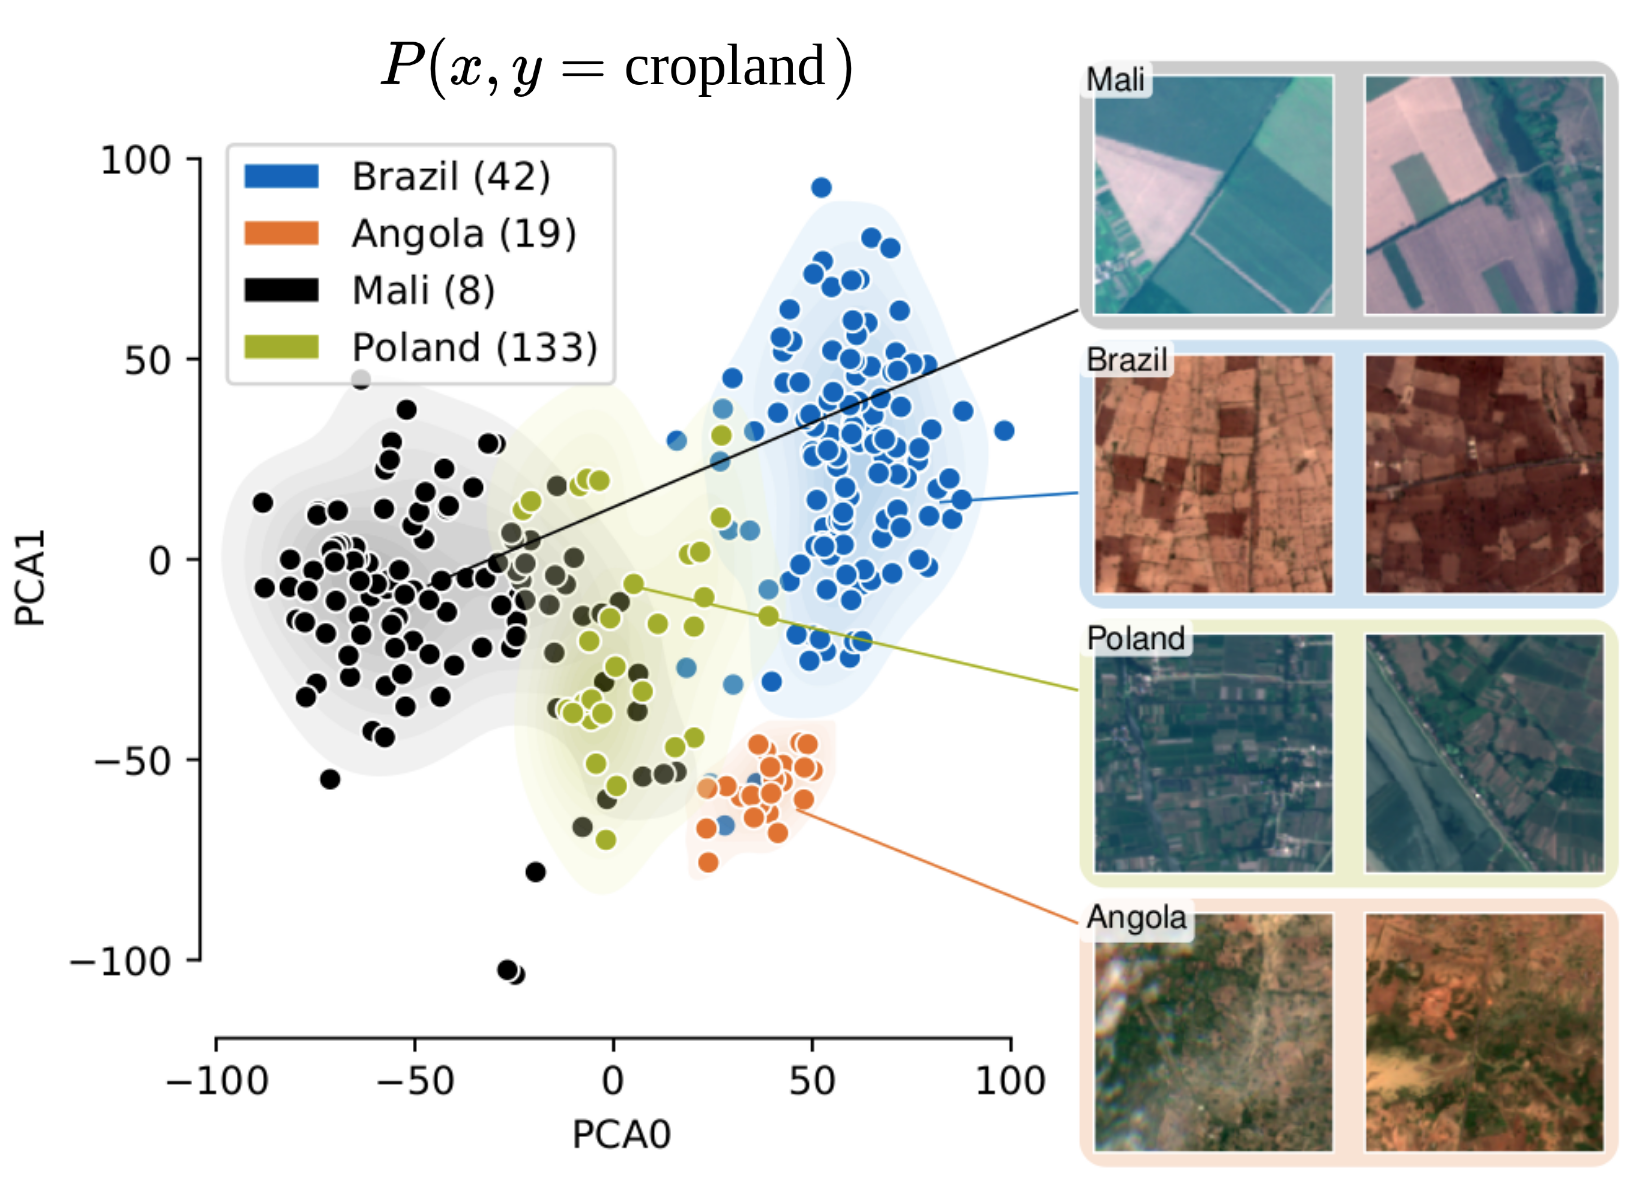
\includegraphics[width=.9\textwidth]{images/Sen12ms_distribution_shift}
%		
%		\scriptsize
%		Figure from
%		
%		\citeapa{Rußwurm, M., Wang, S., Körner, M., \& Lobell, D. (2020). Meta-learning for few-shot land cover classification. In Proceedings of the ieee/cvf conference on computer vision and pattern recognition workshops (pp. 200-201).}
%		
%		\scriptsize
%		Data from
%		
%		\citeapa{Schmitt, M., Hughes, L. H., Qiu, C., \& Zhu, X. X. (2019). SEN12MS--A Curated Dataset of Georeferenced Multi-Spectral Sentinel-1/2 Imagery for Deep Learning and Data Fusion. arXiv preprint arXiv:1906.07789.}
%	\end{frame}

	\begin{frame}{Improve on the target Task/Domain}
		
		Option 1) Just train on target data {\scriptsize (we will call "random initialization")}
		
		\vspace{2em}
		
		\begin{tikzpicture}
		
		{\color{perle}
		\node(ds) at (0,0){$D \iidsim P(\mathcal{X} \times \mathcal{Y})$};
		\node at (-1,-1)(dstrain){$D_\text{train}$};
		\node at (1,-1)(dstest){$D_\text{test}$};
		
		\draw[-Stealth](ds) --node[midway, left=1em, font=\tiny, name=labelsplit]{random split} (dstrain);
		\draw[-Stealth](ds) -- (dstest);
		
		\node[draw, rounded corners, fit=(ds)(dstrain)(dstest)(labelsplit), label={above: Source Task/Domain\phantom{g}}]{};
		}
		
		\begin{scope}[xshift=5cm]
		\node(Q) at (0,0){$D \iidsim Q(\mathcal{X} \times \mathcal{Y})$};
		\node at (-1,-1)(dsqtrain){$D_\text{train}$};
		\node at (1,-1)(dsqtest){$D_\text{test}$};
		\end{scope}
		
		\node[below=of dsqtrain, label={[font=\tiny]left:train model}] (weightsq) {$f_\theta$};
		\draw[-Stealth] (dsqtrain) -- (weightsq);
		
		\draw[-Stealth](Q) --node[midway, left=0.5em, font=\tiny, name=labelqsplit]{random split} (dsqtrain);
		\draw[-Stealth](Q) -- (dsqtest);
		
		\node[draw, rounded corners, fit=(Q)(dsqtrain)(dsqtest)(labelqsplit), label={above: Target Task/Domain}]{};
		
		\node[below=of dsqtest] (oodloss) {$\mathcal{L}$};
%		\node[below=0em of oodloss, text width=3cm, font=\scriptsize](oodlabel){"out-of-domain" or \\ "out-of-distribution" \\ generalization};
%		
		\draw[-Stealth] (weightsq) -- node[midway,above,font=\tiny]{compare with $f_Q(\cdot)$} (oodloss);
		\draw[-Stealth] (dsqtest) -- (oodloss);
		
		\end{tikzpicture}
	\end{frame}


	\begin{frame}{Improve on the target Task/Domain}
		
		Option 2) "Pretrain" on Source finetune on Target 
		
		\vspace{2em}
		
		\begin{tikzpicture}
			\node(ds) at (0,0){$D \iidsim P(\mathcal{X} \times \mathcal{Y})$};
			\node at (-1,-1)(dstrain){$D_\text{train}$};
			\node at (1,-1)(dstest){$D_\text{test}$};
			
			\draw[-Stealth](ds) --node[midway, left=1em, font=\tiny, name=labelsplit]{random split} (dstrain);
			\draw[-Stealth](ds) -- (dstest);
			
			\node[draw, rounded corners, fit=(ds)(dstrain)(dstest)(labelsplit), label={above: Source Task/Domain\phantom{g}}]{};
			
			\node[below=of dstrain, label={[font=\tiny]left:train model}] (weights) {$f_\theta$};
			\draw[-Stealth] (dstrain) -- (weights);
			
%			\node[below=of dstest] (testloss) {$\mathcal{L}_\text{in}$};
			\draw[Stealth-] (dstest) -- node[midway, right, font=\tiny]{generalize in dist.} (weights);
			\draw[-Stealth] (weights) -- node[midway,above,font=\tiny]{initialize} (weightsq);
			
		\begin{scope}[xshift=5cm]
		\node(Q) at (0,0){$D \iidsim Q(\mathcal{X} \times \mathcal{Y})$};
		\node at (-1,-1)(dsqtrain){$D_\text{train}$};
		\node at (1,-1)(dsqtest){$D_\text{test}$};
		\end{scope}
		
		\node[below=of dsqtrain] (weightsq) {$f_\theta$};
		\draw[-Stealth] (dsqtrain) -- node[midway, left, font=\tiny]{finetune} (weightsq);
		
		\draw[-Stealth](Q) --node[midway, left=0.5em, font=\tiny, name=labelqsplit]{random split} (dsqtrain);
		\draw[-Stealth](Q) -- (dsqtest);
		
		\node[draw, rounded corners, fit=(Q)(dsqtrain)(dsqtest)(labelqsplit), label={above: Target Task/Domain}]{};
		
		\node[below=of dsqtest] (oodloss) {$\mathcal{L}$};
		%		\node[below=0em of oodloss, text width=3cm, font=\scriptsize](oodlabel){"out-of-domain" or \\ "out-of-distribution" \\ generalization};
		%		
		\draw[-Stealth] (weightsq) -- node[midway,above,font=\tiny]{compare with $f_Q(\cdot)$} (oodloss);
		\draw[-Stealth] (dsqtest) -- (oodloss);
		
		\end{tikzpicture}
		
%		\vfill
%		\only<1>{
%			{	\scriptsize
%				Side Note: "Transfer Learning aims to help improve the learning of the target predictive function $f_Q(\cdot)$ for the target domain using the knowledge in $\mathcal{D}_s$ and $\mathcal{T}_s$ where $\mathcal{D}_s \neq \mathcal{D}_t$ and $\mathcal{T}_s \neq \mathcal{T}_t$" \par
%			}
%			\vspace{.5em}
%				\citeapa{Qiang Yang; Yu Zhang, Wenyuan Dai; Sinno Jialin Pan (Editors) (2020). Transfer learning. Cambridge University Press. DOI 9781139061773}
%		}
%		\only<2>{
%			{	\scriptsize
%				Side-Note 2: Examples of recent methods for crop type mapping.
%				
%				\vspace{.5em}
%				
%				\citeapa{Lucas, B., Pelletier, C., Schmidt, D., Webb, G. I., \& Petitjean, F. (2021). A Bayesian-inspired, deep learning-based, semi-supervised domain adaptation technique for land cover mapping. Machine Learning, 1-33.}
%				
%				\vspace{.5em}
%				
%				\citeapa{Joachim Nyborg, Charlotte Pelletier, Sébastien Lefèvre \& Ira Assent (2021). TimeMatch: Unsupervised Cross-Region Adaptation by Temporal Shift Estimation. Preprint}
%			}
%		}
	\end{frame}

	\begin{frame}{Improve on the target Task/Domain}
		
		Option 3) ML framework that allows not ident. joint dists \\
		
		and in particular Model-Agnostic Meta-Learning \\ {\scriptsize (Finn et al., 2017)}.
		
		\vspace{1em}
		
		\begin{tikzpicture}
		\node(ds) at (0,0){$D \iidsim P_i(\mathcal{X} \times \mathcal{Y})$};
		\node at (-1,-1)(dstrain){$D_\text{train}$};
		\node at (1,-1)(dstest){$D_\text{test}$};
		
		\draw[-Stealth](ds) --node[midway, left=1em, font=\tiny, name=labelsplit]{random split} (dstrain);
		\draw[-Stealth](ds) -- (dstest);
		
		\node[draw, rounded corners, fit=(ds)(dstrain)(dstest)(labelsplit), label={above: Source Tasks/Domains\phantom{g}}](box){};
		\foreach \d in {0.05,0.1,0.15,0.2}
		{
			\draw[draw, rounded corners] ($(box.south west)+(\d,-\d)$) -- ($(box.south east)+(\d,-\d)$) -- ($(box.north east)+(\d,-\d)$);
		}
		
		\node[below=of dstrain] (weights) {$f_{\theta_i}$};
		\draw[-Stealth] (dstrain) -- node[midway, left, font=\tiny]{finetune} (weights);
		
		%
					
		\node[left=of weights, label={[font=\tiny]below:meta-weights}] (metaweights) {$\theta^\ast$};
		\draw[-Stealth] (metaweights) --node[midway, below, font=\tiny]{initialize} (weights);
		
		%			\node[below=of dstest] (testloss) {$\mathcal{L}_\text{in}$};
		\draw[Stealth-] (dstest) -- node[midway, right, font=\tiny, name=testgen]{generalize in dist.} (weights);

		\visible<2>{
			\draw[-Stealth, draw=EPFLred] (testgen) to [bend left=45] node[midway, below right, font=\tiny, text=EPFLred, text width=3cm]{update meta weights \\ over a batch of tasks/domains} (metaweights);
%			\draw[-Stealth]($(dstrain.south)+(.1,-.1)$) -- ($(weights.north)+(.1,-.05)$);
%			\draw[-Stealth]($(dstrain.south)+(.2,-.2)$) -- ($(weights.north)+(.2,-.1)$);
%			
%			\draw[-Stealth]($(weights.north east)+(.1,0)$) -- ($(dstest.south west)+(.1,0)$);
%			\draw[-Stealth]($(weights.north east)+(.2,0)$) -- ($(dstest.south west)+(.2,0)$);
		}	
		
		\only<1-2>{
			\color{perle}
		}
		\only<3->{
			\color{black}
			\draw[-Stealth] (metaweights) to[bend right=10] node[midway,above,font=\tiny]{initialize} (weightsq);
		}
	
		
		\begin{scope}[xshift=5cm]
		\node(Q) at (0,0){$D \iidsim Q_j(\mathcal{X} \times \mathcal{Y})$};
		\node at (-1,-1)(dsqtrain){$D_\text{train}$};
		\node at (1,-1)(dsqtest){$D_\text{test}$};
		\end{scope}
		
		\node[below=of dsqtrain] (weightsq) {$f_\theta$};
		\draw[-Stealth] (dsqtrain) -- node[midway, left, font=\tiny]{finetune} (weightsq);
		
		\draw[-Stealth](Q) --node[midway, left=0.5em, font=\tiny, name=labelqsplit]{random split} (dsqtrain);
		\draw[-Stealth](Q) -- (dsqtest);
		
		\node[draw, rounded corners, fit=(Q)(dsqtrain)(dsqtest)(labelqsplit), label={above: Target Tasks/Domains}](box){};
		
		\foreach \d in {0.05,0.1,0.15,0.2}
		{
			\draw[draw, rounded corners] ($(box.south west)+(\d,-\d)$) -- ($(box.south east)+(\d,-\d)$) -- ($(box.north east)+(\d,-\d)$);
		}
		
		\node[below=of dsqtest] (oodloss) {$\mathcal{L}$};
		%		\node[below=0em of oodloss, text width=3cm, font=\scriptsize](oodlabel){"out-of-domain" or \\ "out-of-distribution" \\ generalization};
		%		
		\draw[-Stealth] (weightsq) -- node[midway,above,font=\tiny]{compare with $f_Q(\cdot)$} (oodloss);
		\draw[-Stealth] (dsqtest) -- (oodloss);
		
		\end{tikzpicture}
		
		\vfill
		\citeapa{Finn, C., Abbeel, P., \& Levine, S. (2017, July). Model-agnostic meta-learning for fast adaptation of deep networks. In International Conference on Machine Learning (pp. 1126-1135). PMLR.}
		
	\end{frame}

	\begin{frame}{A Visual Comparison}
		
		\tikzfading[name = dist fading,
		inner color = transparent!0,
		outer color = transparent!100]
		
		\tikzstyle{dist} = [font=\tiny, path fading = dist fading, inner sep=2em]
		
		
		\scriptsize
		\begin{columns}[t]
%			\column{.33\textwidth}
%			Random Initialization
%			
%			\begin{tikzpicture}[scale=0.5]
%			
%				\visible<1-7>{
%					\node (metaparameters) at (1,0){$\theta^\text{rand}$};
%					
%					\node[dist, inner color=perle, color=perle](a) at (3,2){$f_{P_1}$};
%					\node[dist, inner color=perle, color=perle](b) at (6,0){$f_{P_2}$};
%					\node[dist, inner color=perle, color=perle](c) at (3,-2){$f_{P_3}$};
%				}
%				
%				\visible<8>{	
%					
%					\node[dist, inner color=perle, color=perle](a) at (3,2){$f_{P_1}$};
%					\node[dist, inner color=perle, color=perle](b) at (6,0){$f_{P_2}$};
%					\node[dist, inner color=perle, color=perle](c) at (3,-2){$f_{P_3}$};
%%					
%					\node (p) at (1,0){$\theta^\text{rand}$};
%					\node[dist, inner color=acier](q) at (6,-3){$f_{Q}$};
%					
%					\draw[-Stealth] (p) -- (q);
%				}
%			\end{tikzpicture}
%			\visible<8>{
%				\textbf{random} baseline
%			}
%		
%			\column{.33\textwidth}
%			Pretrained Initialization
%			
%			\begin{tikzpicture}[scale=0.5]
%			
%				\visible<1-7>{
%					\node[dist, inner color=rouge](a) at (3,2){$f_{P_1}$};
%					\node[dist, inner color=rouge](b) at (6,0){$f_{P_2}$};
%					\node[dist, inner color=rouge](c) at (3,-2){$f_{P_3}$};
%				}
%			
%				\visible<1-2>{
%					\node (p) at (1,0){$\theta^\text{rand}$};
%					
%					\draw[-Stealth] (p) -- (a.center);
%					\draw[-Stealth] (p) -- (b.center);
%					\draw[-Stealth] (p) -- (c.center);
%				}
%			
%				\visible<2>{
%					\draw[-Stealth, rouge] (a.center) to[bend left=25] (p);
%					\draw[-Stealth, rouge] (b.center) to[bend left=15] (p);
%					\draw[-Stealth, rouge] (c.center) to[bend left=25] (p);	
%				}
%			
%				\visible<3>{
%					\node (p) at (1,0){$\theta^\text{rand.}$};
%					\node (p2) at (4,0){$\theta^\text{pretr.}$};
%					\draw[-Stealth] (p) -- node[midway, above, font=\tiny]{SGD} (p2);
%				}
%				
%				\visible<7>{
%					\node (p) at (4,0){$\theta^\text{pretr.}$};
%					\draw[-Stealth] (p) -- (a.center);
%					\draw[-Stealth] (p) -- (b.center);
%					\draw[-Stealth] (p) -- (c.center);
%				}
%			
%				\visible<8>{	
%					
%					\node[dist, inner color=perle, color=perle](a) at (3,2){$f_{P_1}$};
%					\node[dist, inner color=perle, color=perle](b) at (6,0){$f_{P_2}$};
%					\node[dist, inner color=perle, color=perle](c) at (3,-2){$f_{P_3}$};
%					
%					\node (p) at (4,0){$\theta^\text{pretrained}$};
%					\node[dist, inner color=acier](q) at (6,-3){$f_{Q}$};
%					
%					\draw[-Stealth] (p) -- (q);
%				}
%				
%			\end{tikzpicture}
%			\visible<8>{
%				Optimized \textbf{to perform} well on source distributions
%				}

			\column{.66\textwidth}
			
				\begin{tikzpicture}
					\node[inner sep=0](a){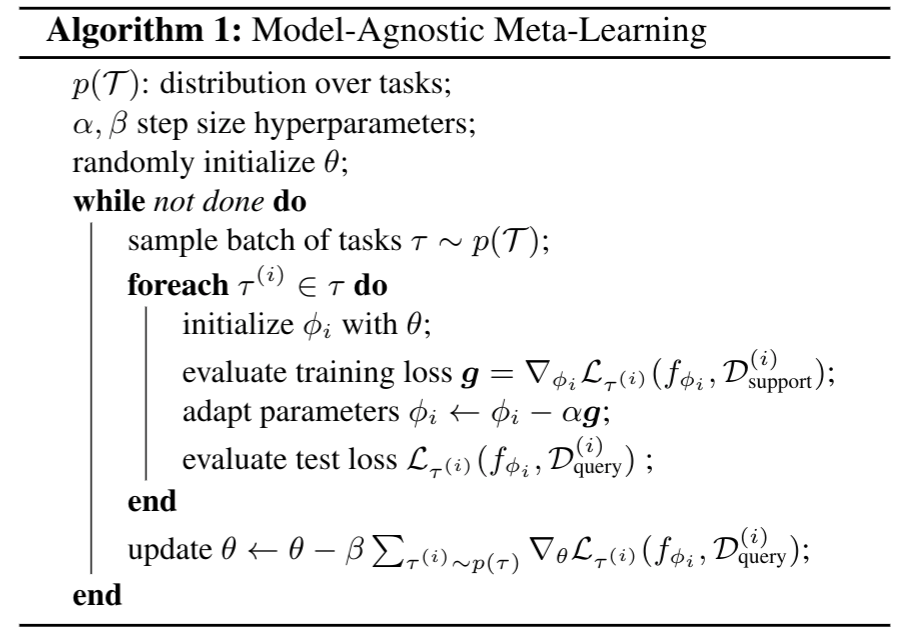
\includegraphics[width=7cm]{maml_algs/maml_alg}};
					
					\visible<1>{
						\node[circle, fill=rouge, xshift=-2.7cm, yshift=0.6cm] at (a.center){};
					}
					\visible<2>{
						\node[circle, fill=rouge, xshift=-2.3cm, yshift=-.43cm] at (a.center){};
					}
					\visible<3>{
						\node[circle, fill=rouge, xshift=-2.3cm, yshift=-.78cm] at (a.center){};
					}
					\visible<4>{
						\node[circle, fill=rouge, xshift=-2.3cm, yshift=-1.12cm] at (a.center){};
					}
					\visible<5>{
						\node[circle, fill=rouge, xshift=-2.7cm, yshift=-1.82cm] at (a.center){};
					}
				\end{tikzpicture}
				
%
			\column{.45\textwidth}
			
			Meta-Learned Initialization
			
			\begin{tikzpicture}[scale=0.5]
			
				\visible<1-6>{
					\node[dist, inner color=rouge](a) at (3,2){$f_{P_1}$};
					\node[dist, inner color=canard](b) at (6,0){$f_{P_2}$};
					\node[dist, inner color=grosseille](c) at (3,-2){$f_{P_3}$};
				}
				
				\visible<2>{
					\node (p) at (1,0){$\theta$};
					
					\draw[-Stealth] (p) -- (a.center);
					\draw[-Stealth] (p) -- (b.center);
					\draw[-Stealth] (p) -- (c.center);

					\draw[-Stealth, rouge] (a.center) to[bend left=25] (p);
					\draw[-Stealth, rouge] (b.center) to[bend left=15] (p);
					\draw[-Stealth, rouge] (c.center) to[bend left=25] (p);	
				}
			
				\visible<3>{
					\node (p) at (1,0){$\theta$};
					
					\node[inner sep=0] (pa) at ($(p)!0.5!(a)$) {$\phi_1$};
					\node[inner sep=0] (pb) at ($(p)!0.5!(b)$) {$\phi_2$};
					\node[inner sep=0] (pc) at ($(p)!0.5!(c)$) {$\phi_3$};
					
					\draw[-Stealth] (p) -- node[midway, left, font=\tiny]{SGD} (pa);
					\draw[-Stealth] (p) -- (pb);
					\draw[-Stealth] (p) -- (pc);
				}
			
				\visible<4-5>{
					\node (p) at (1,0){$\theta$};
					
					\node[inner sep=0] (pa) at ($(p)!0.5!(a)$) {$\phi_1$};
					\node[inner sep=0] (pb) at ($(p)!0.5!(b)$) {$\phi_2$};
					\node[inner sep=0] (pc) at ($(p)!0.5!(c)$) {$\phi_3$};
					
					\draw[-Stealth] (pa) -- (a.center);
					\draw[-Stealth] (pb) -- (b.center);
					\draw[-Stealth] (pc) -- (c.center);
				}
			
				\visible<5>{
					\draw[-Stealth, rouge] (a.center) to[bend left=25] (pa);
					\draw[-Stealth, rouge] (b.center) to[bend left=25] (pb);
					\draw[-Stealth, rouge] (c.center) to[bend left=25] node[midway, left, font=\tiny]{inner loop} (pc);
				
					\draw[-Stealth, rouge] (pa) to (p);
					\draw[-Stealth, rouge] (pb) to (p);
					\draw[-Stealth, rouge] (pc) to node[midway, left, font=\tiny]{outer loop} (p);
				}
			
				\visible<6>{
					\node (p) at (1,0){$\theta$};
					\node (pa) at (4,0){$\theta$};
					\draw[-Stealth] (p) -- (pa);
					
%					\node[inner sep=0em] (pa) at ($(p)!0.75!(a)$) {$\phi_1$};
%					\node[inner sep=0em] (pb) at ($(p)!0.75!(b)$) {$\phi_2$};
%					\node[inner sep=0em] (pc) at ($(p)!0.75!(c)$) {$\phi_3$};
%					
%					\draw[-Stealth] (p) -- (pa);
%					\draw[-Stealth] (p) -- (pb);
%					\draw[-Stealth] (p) -- (pc);
%					
%					\draw[-Stealth] (pa) -- (a.center);
%					\draw[-Stealth] (pb) -- (b.center);
%					\draw[-Stealth] (pc) -- (c.center);
				}
			
				\visible<7->{	
					
					\node[dist, inner color=perle, color=perle](a) at (3,2){$f_{P_1}$};
					\node[dist, inner color=perle, color=perle](b) at (6,0){$f_{P_2}$};
					\node[dist, inner color=perle, color=perle](c) at (3,-2){$f_{P_3}$};
					
					\node (p) at (4,0){$\theta$};
					\node[dist, inner color=acier](q) at (6,-3){$\phi$};
					
					\draw[-Stealth] (p) -- (q.center);
				}
				
			\end{tikzpicture}
			\visible<7->{
			Optimized \textbf{to adapt} well to source distributions
			}
			\visible<8>{
				
				\vspace{1em}
				
				while regular \textbf{pretraining} is optimized \textbf{to perform} well on source distributions.
				}
			
		\end{columns}

	\end{frame}

	\begin{frame}[plain]
		\vfill
		\Large \centering
			Experiments
		\vfill
	\end{frame}
	
	\begin{frame}{Deepglobe Land Cover Classification}
		\begin{columns}
			\column{.4\textwidth}
			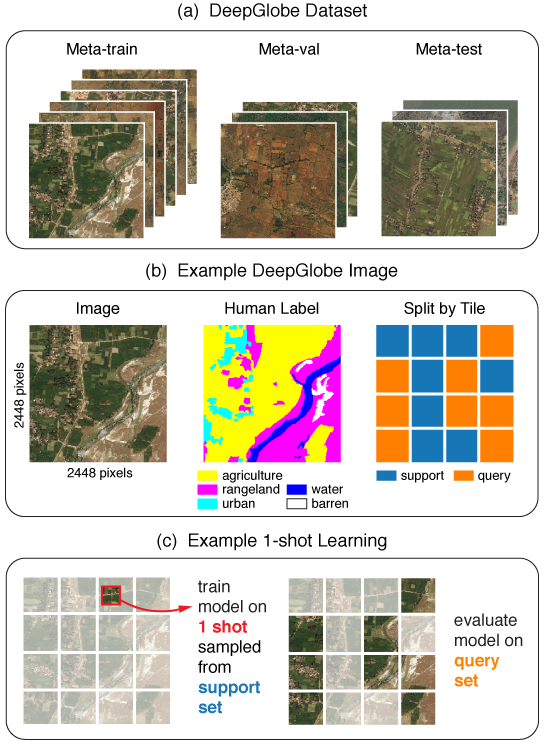
\includegraphics[width=\textwidth]{deepglobe/deepglobe_dataset}
			\column{.6\textwidth}
			
			\visible<2->{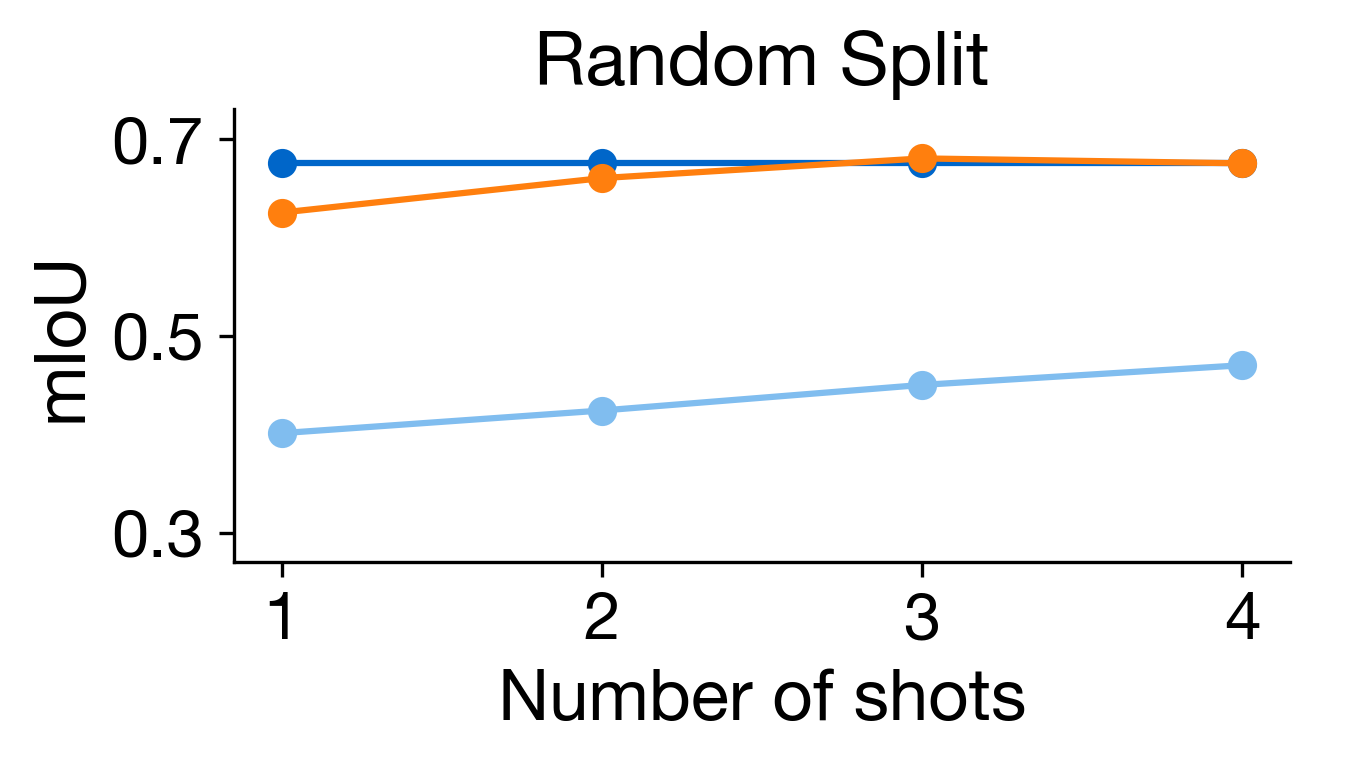
\includegraphics[height=1.8cm]{deepglobe/deepglobe_results_shots_1}}
			\visible<5->{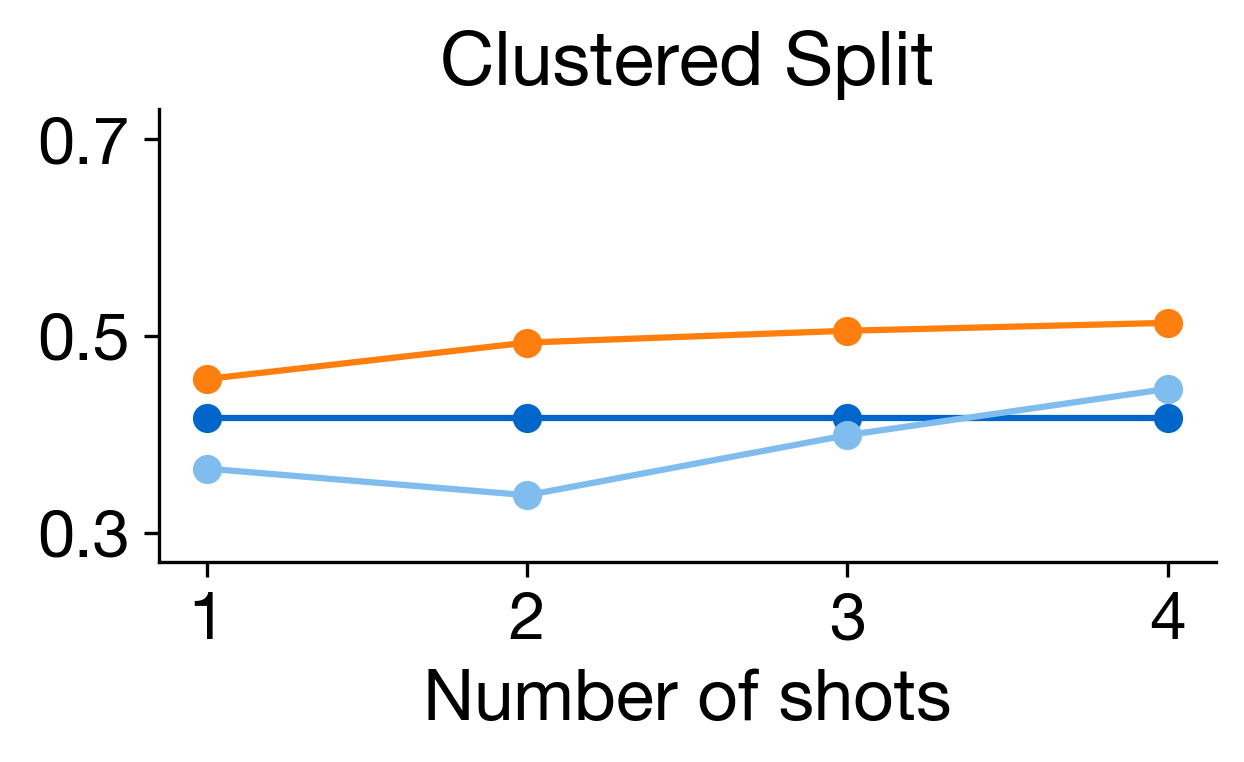
\includegraphics[height=1.8cm]{deepglobe/deepglobe_results_shots_2}}
				
			\visible<3->{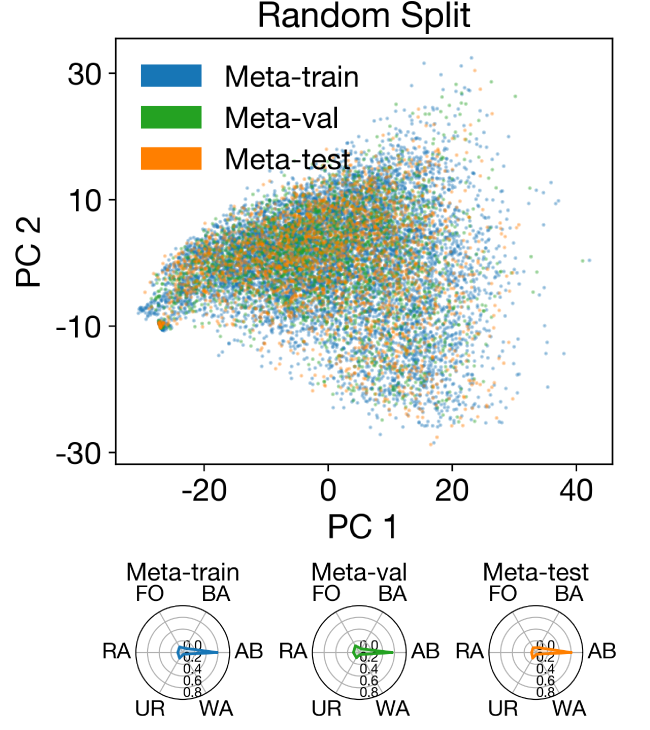
\includegraphics[height=3.7cm]{deepglobe/deepglobe_results_pca_1}}
			\visible<4->{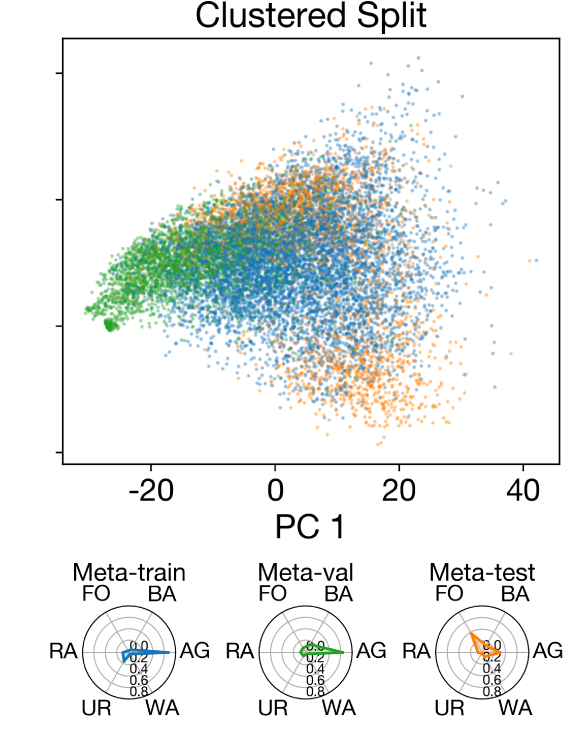
\includegraphics[height=3.7cm]{deepglobe/deepglobe_results_pca_2}}
				
			\visible<2>{
				\begin{tikzpicture}[xscale=1.2]
				\node[fill=tumbluelight,font=\tiny,text=white] at (0,0){random};
				\node[fill=tumbluedark,font=\tiny,text=white] at (1,0){pretrained};
				\node[fill=tumorange,font=\tiny,text=white] at (2,0){MAML};
				\end{tikzpicture}
			}
			
		\end{columns}
	
		\vspace{1em}
		
		\citeapa{Rußwurm, M., Wang, S., Körner, M., \& Lobell, D. (2020). Meta-learning for few-shot land cover classification. In Proceedings of the ieee/cvf conference on computer vision and pattern recognition workshops (pp. 200-201).}
		
	\end{frame}

	\begin{frame}{Sen12MS ---  Land Cover Classification}
				\begin{tikzpicture}
		\node[label={[font=\small, node distance=0em]above:all Sen12MS regions}](a) at (0,0){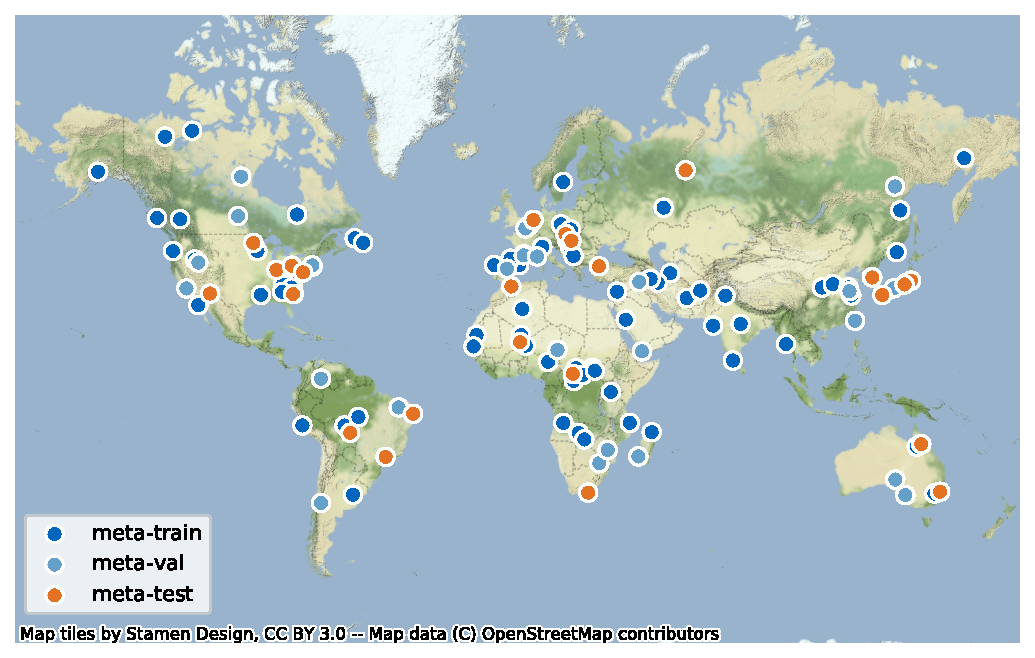
\includegraphics[height=3.5cm]{images/sen12ms_metasplit}};
		\node[right=of a, label={[font=\small, node distance=0em]above:one region split in train/test}]{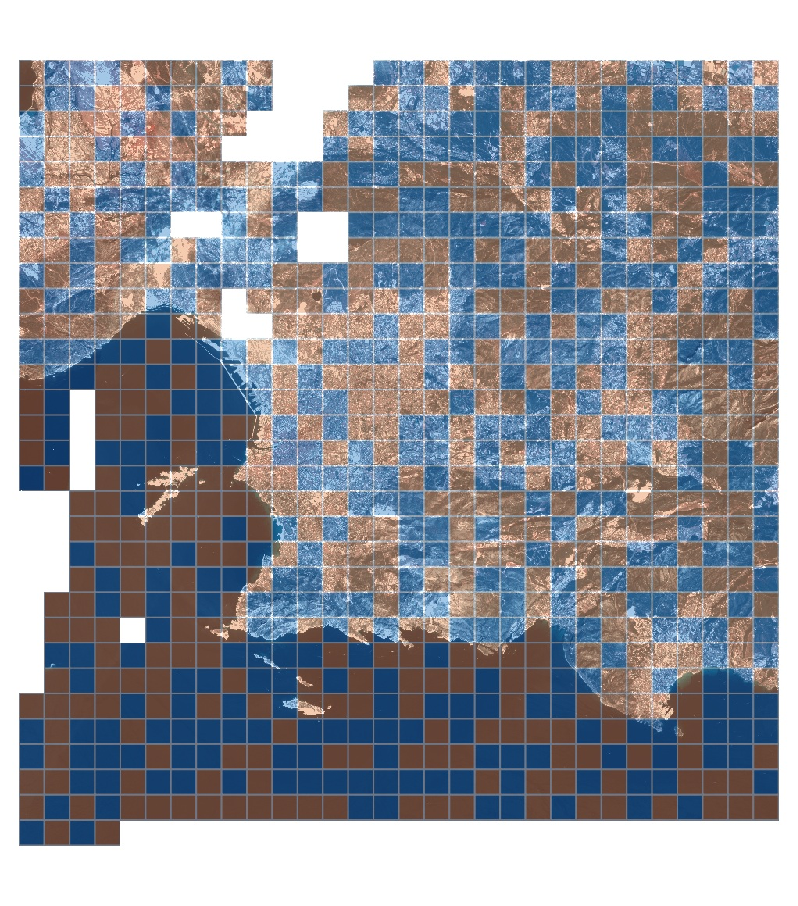
\includegraphics[height=3.5cm]{images/rgb_fold_overlayed}};
		\end{tikzpicture}
		
		\citeapa{Schmitt, M., Hughes, L. H., Qiu, C., \& Zhu, X. X. (2019). SEN12MS--A Curated Dataset of Georeferenced Multi-Spectral Sentinel-1/2 Imagery for Deep Learning and Data Fusion. arXiv preprint arXiv:1906.07789.}
	\end{frame}

%	\begin{frame}
%		\tikzstyle{labelstyle} = [font=\tiny\sffamily]
%		
%		 		\begin{tikzpicture}
%		
%		 		\newcommand{\traintaska}{
%		 			\begin{tikzpicture}[xscale=.75]
%		 				\node[label={[labelstyle]below=0em:forest}] at (0,0) {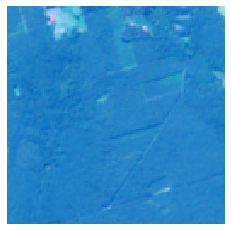
\includegraphics[width=.7cm]{figures/sen12ms-2d-losses/pretrained/0/traintask1/summer-56-Forests-p53br.png}};
%		 				\node[label={[labelstyle]below:grassland}] at (1,0) {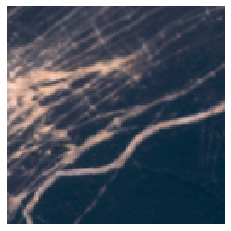
\includegraphics[width=.7cm]{figures/sen12ms-2d-losses/pretrained/0/traintask1/summer-56-Grassland-p37tl.png}};
%		 				\node[label={[labelstyle]below:savanna}] at (2,0) {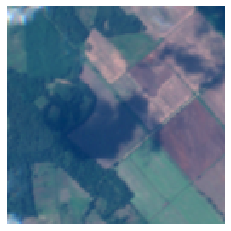
\includegraphics[width=.7cm]{figures/sen12ms-2d-losses/pretrained/0/traintask1/summer-56-Savanna-p168br.png}};
%		 				\node[label={[labelstyle]below:urban}] at (3,0) {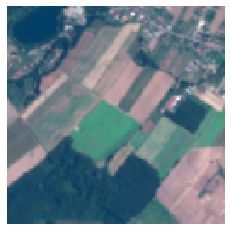
\includegraphics[width=.7cm]{figures/sen12ms-2d-losses/pretrained/0/traintask1/summer-56-Urban_Build-up-p417tl.png}};
%		 			\end{tikzpicture}
%		 		}
%				\hspace{-2cm}
%		 		\node[label={[font=\scriptsize\sffamily, yshift=-1em]above:MAML}](a){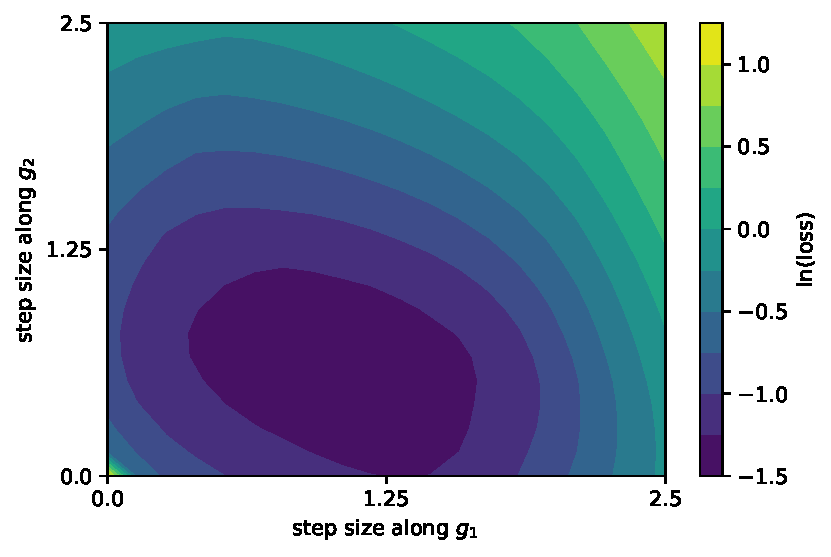
\includegraphics[width=4cm]{figures/sen12ms-2d-losses/maml/0/loss_surface}};
%		 		\node[label={[font=\scriptsize\sffamily, yshift=-1em]above:pre-trained}, right=0em of a](pretrained){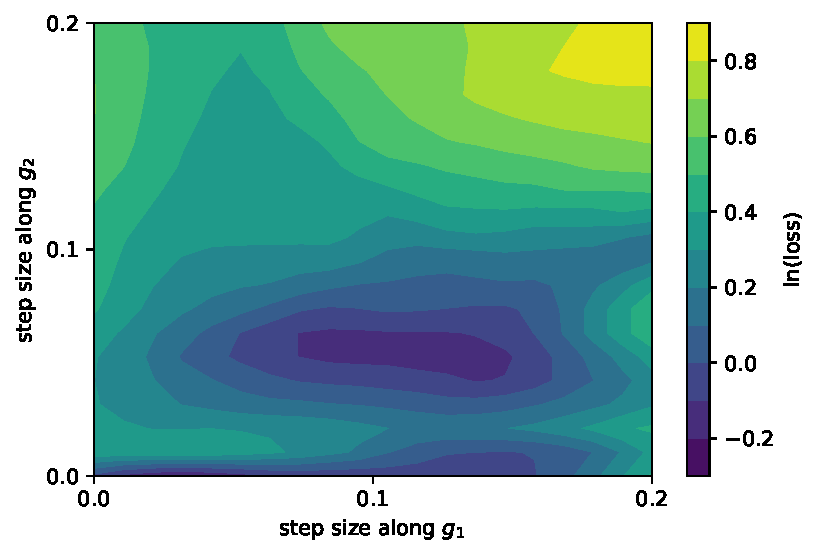
\includegraphics[width=4cm]{figures/sen12ms-2d-losses/pretrained/0/loss_surface}};
%		 		\node[label={[font=\scriptsize\sffamily, yshift=-1em]above:random}, right=0em of pretrained](random){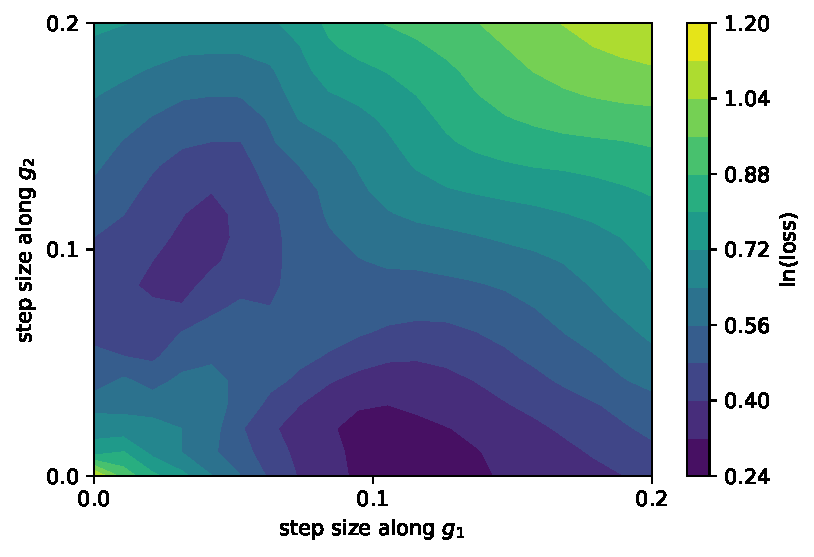
\includegraphics[width=4cm]{figures/sen12ms-2d-losses/random/0/loss_surface}};
%%		 		\node[below=0em of pretrained]{\traintaska};
%%		
%		 		\end{tikzpicture}
%	\end{frame}

	
%	\begin{frame}[plain]
%		\centering
%		\hfill
%		\Large
%		
%		Experiments
%		
%		\hfill
%	\end{frame}


	\begin{frame}{Sen12MS -- Few-Shot Performance}
		
		{\scriptsize Model: 7 stacked CNN layers 64 x 3 x 3 kernels + BN + ReLU + max-pooling}
		
		Classification
		\begin{tikzpicture}
		\begin{axis}[
		height=3cm,
		width=\textwidth,
		xtick={0,1,2,3,4,5,6,7,8,9,10},
		legend style={at={(0.5,1)},anchor=south},
		legend columns=3,
		ylabel={accuracy},
		xlabel=shots,
		ymin=0,
		ymax=1,
		ymajorgrids,
		]
		\addplot[mamlcolor, mark = *] table [x=index, y=accuracy, col sep=comma] {figures/sen12ms_classification/4-way/maml.csv};
		\addlegendentry{maml}
		\addplot[pretrainedcolor, mark = *] table [x=index, y=accuracy, col sep=comma] {figures/sen12ms_classification/4-way/pretrained.csv};
		\addlegendentry{pretrained}
		\addplot[randomcolor, mark = *] table [x=index, y=accuracy, col sep=comma] {figures/sen12ms_classification/4-way/random.csv};
		\addlegendentry{random}
		\end{axis}
		\end{tikzpicture}
		
		Segmentation
		\begin{tikzpicture}
		\begin{axis}[
		height=3cm,
		width=\textwidth,
		xtick={0,1,2},
		xticklabels={0,1,5},
%		xmax=6,
		legend style={at={(0.5,1)},anchor=south},
		legend columns=3,
		ylabel={accuracy},
		xlabel=shots,
		ymin=0,
		ymax=1,
		ymajorgrids,
		]
		\addplot[mamlcolor, mark = *] table [x=index, y=accuracy, col sep=comma] {figures/sen12ms_segmentation/maml.csv};
		\addlegendentry{maml}
		\addplot[pretrainedcolor, mark = *] table [x=index, y=accuracy, col sep=comma] {figures/sen12ms_segmentation/pretrained.csv};
		\addlegendentry{pretrained}
		\addplot[randomcolor, mark = *] table [x=index, y=accuracy, col sep=comma] {figures/sen12ms_segmentation/random.csv};
		\addlegendentry{random}
		\end{axis}
		\end{tikzpicture}
		
		\citeapa{Rußwurm, M., Wang, S., Körner, M., \& Lobell, D. (2020). Meta-learning for few-shot land cover classification. In Proceedings of the ieee/cvf conference on computer vision and pattern recognition workshops (pp. 200-201).}
		
	\end{frame}

	\begin{frame}{Modis Time Series Classification}
		\centering
%		\begin{columns}
%			\column{.4\textwidth}
%				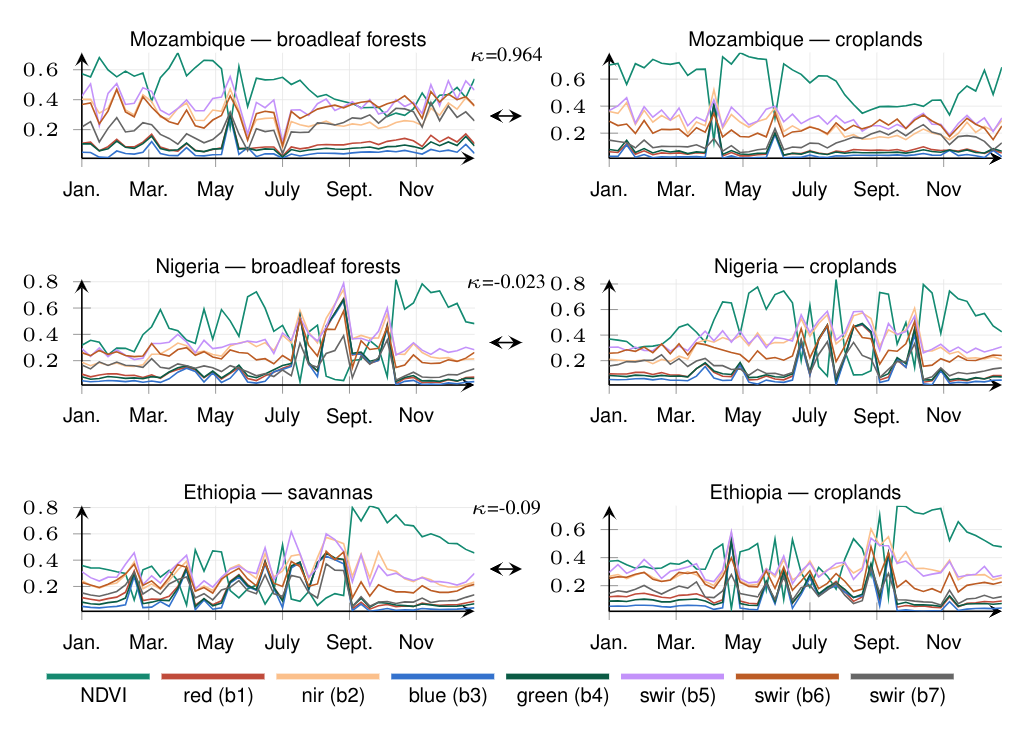
\includegraphics[width=.49\textwidth]{igarss2020/examples}
				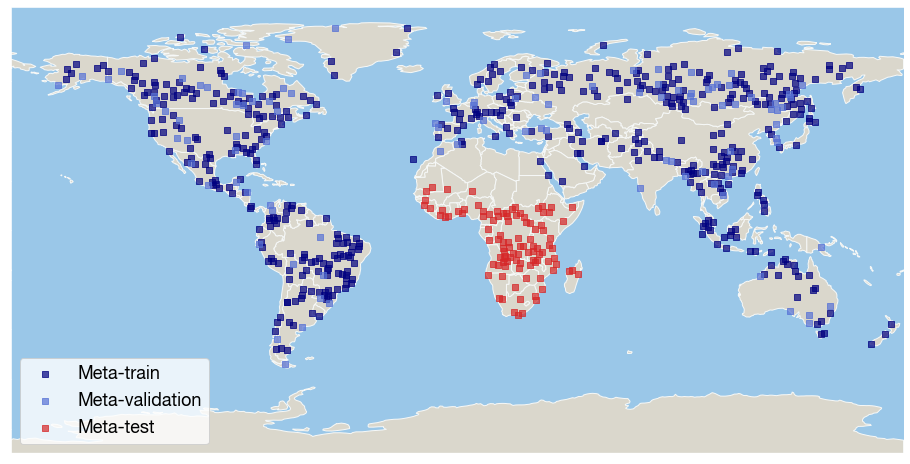
\includegraphics[width=.75\textwidth]{igarss2020/modis_task_map}
%				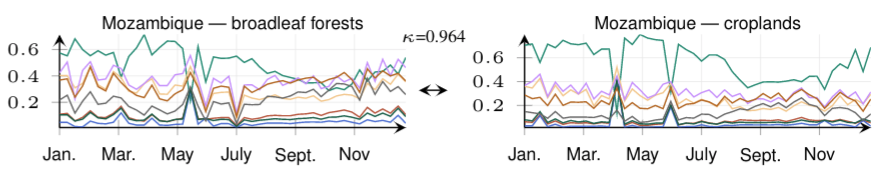
\includegraphics[height=1.5cm]{igarss2020/modis_task}
%			\column{.6\textwidth}
				
		\vfill
		
		1-shot 2-way, 515 meta-test tasks from Africa
%		\end{columns}

		\citeapa{Wang, S., Rußwurm, M., Körner, M., \& Lobell, D. B. Meta-Learning For Few-Shot Time Series Classification. In IGARSS 2020-2020 IEEE International Geoscience and Remote Sensing Symposium (pp. 7041-7044). IEEE.}
	\end{frame}

	\begin{frame}{Challenging Problem: Mixed results}
		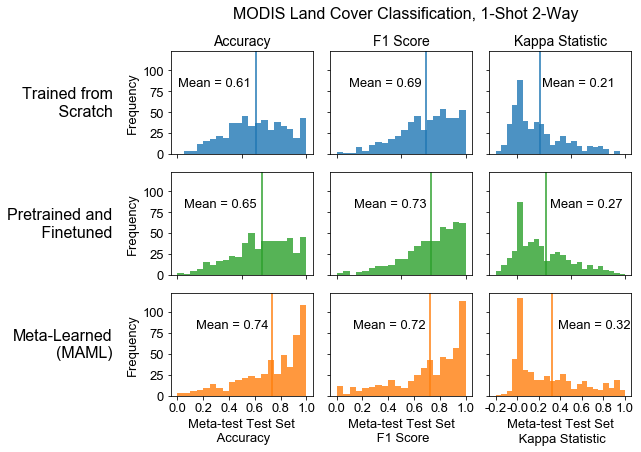
\includegraphics[width=\textwidth]{igarss2020/modis_africa_histograms_narrow}
	\end{frame}

	\begin{frame}{Summary: When to Transfer?}
		
%		when source and target task/domains...
%		\begin{itemize}
%			\item are similar: regular machine learning is sufficient
%			\item are related: transfer learning is beneficial 
%			\item are not related: brute-force transfer may be unsuccessful.
%		\end{itemize}
	
		\vspace{1em}
		"When to transfer?" of Yang et al., (2020). 
		\vspace{1em}
		\begin{itemize}
			\item<1-> If distributions are too similar, transfer learning is not necessary. (e.g. DeepGlobe, unclustered)
			\item<2-> if distributions are related, transfer learning is effective (e.g. Sen12MS)
			\item<3-> If they are to different, there is no common knowledge to be learned. (e.g. Africa-testset: in Modis Time Series)
		\end{itemize} 
	
		\vfill
		
		\citeapa{Pan, S. J., \& Yang, Q. (2009). A survey on transfer learning. IEEE Transactions on knowledge and data engineering, 22(10), 1345-1359.}
		\citeapa{Qiang Yang; Yu Zhang, Wenyuan Dai; Sinno Jialin Pan (Editors) (2020). Transfer learning. Cambridge University Press. DOI 9781139061773}
	\end{frame}

%	\begin{frame}{Summary MAML Experiments}
%		
%%		\begin{columns}[t]
%%			\column{.5\textwidth}
%%				In General
%%				\begin{itemize}
%%					\item Relaxing identical distribution assumption is important!
%%					\item On any geographic data, joint data distributions change
%%					\item in practice, we always train and test on other domains and tasks
%%					\item the question for algorithm designs is how different are these domains/tasks?
%%				\end{itemize}
%%			\column{.5\textwidth}
%				Model-Agnostic Meta Learning
%				\begin{itemize}
%					\item<1-> was effective in some cases (Sen12MS). Not in others (DeepGlobe, Time Series Classification)
%					\item<2-> tailored towards few-shot problems while we often have many data shots available 
%					\item<3-> implementation-wise challenging (2nd order gradients), batching the task/domains in a certain way.
%					\item<4-> Newer approaches have been proposed (MAML++, ProtoMAML, etc)
%				\end{itemize}
%%		\end{columns}
%
%%		\vspace{1em}
%%		
%%		how to integrate task/domain specific information?
%%		\begin{itemize}
%%			\item \citeapa{Tseng, G., Kerner, H., Nakalembe, C., \& Becker-Reshef, I. (2021). Learning To Predict Crop Type From Heterogeneous Sparse Labels Using Meta-Learning. In Proceedings of the IEEE/CVF Conference on Computer Vision and Pattern Recognition (pp. 1111-1120).}
%%			\item \citeapa{Tseng, G., Zvonkov, I., Nakalembe, C. L., \& Kerner, H. (2021). CropHarvest: A global dataset for crop-type classification.}
%%		\end{itemize}
%%	
%
%
%	\end{frame}

	\begin{frame}{Outlook}
%						In General

		
	
		\begin{columns}[t]
			\column{.5\textwidth}
			
				\begin{itemize}
					\item<1-> Out-of-distribution generalization remains challenging. 
					\item<2-> Few-shot meta-learning well-suited for some cases (i.e., many uniformly distributed datasets around the globe).
					\item<3-> We may need to decide on the learning-framework on a case by case basis
				\end{itemize}
			
			\column{.5\textwidth}
			
			\visible<3->{
				Marine Litter Detection
				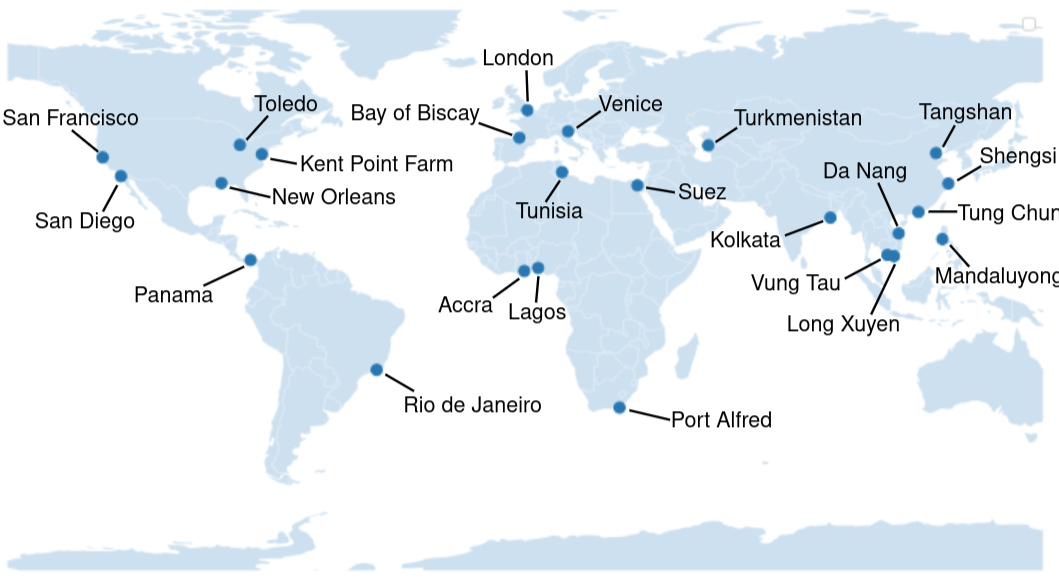
\includegraphics[width=\textwidth]{figures/oceans_map}
				\includegraphics[width=\textwidth]{figures/oceans_predictions}
				\citeapa{Mifdal, J., Longépé, N., and Rußwurm, M. (2021) Towards detecting floating objects on a global scale with learned spatial features using Sentinel 2, ISPRS Ann. Photogramm. Remote Sens. Spatial Inf. Sci., V-3-2021, 285–293.}
		}
			
%			\column{.5\textwidth}
%			Hydrological Modeling
%			\includegraphics[width=\textwidth]{images/camels}
%			
%			\citeapa{A. Newman, K. Sampson, M.P. Clark, A. Bock, and R.J. Viger, and D. Blodgett, 2014: A large-sample watershed-scale hydrometeorological dataset for the contiguous USA. Boulder, CO: UCAR/NCAR. doi:10.5065/D6MW2F4D}
		\end{columns}
	
		\vspace{1cm}
		
		\visible<4>{
			\begin{tikzpicture}[node distance=0.5em]
				\node (a) {what features?};
				
				\node[right=of a] (b) {what DL models?};
				\node[right=of b] (c) {what learning algorithms?};
				\draw[-Stealth] (a) -- (b);
				\draw[-Stealth] (b) -- (c);
			\end{tikzpicture}
		}
	
	\end{frame}

	\begin{frame}[plain]{Thank you!}
		
		
		\pgfdeclareimage[width=1.1\paperwidth]{endgraphic}{epfl/tourbillon}
		%\pgfdeclareimage[width=3cm]{epfllogo}{\@titlepagelogo}
		
		\begin{picture}(0,0)
		
		\put(-50,-253){%
			\pgfuseimage{endgraphic}
		}
	
		\end{picture}
		
		
		\begin{tikzpicture}
%			\node(node name) {\includegraphics[width=1.3\textwidth]{epfl/tourbillon}};
			
			\node[text width=3cm, fill=rouge, text=white, inner sep=0.5cm, font=\bfseries\Large, rounded corners] at (2,3){
				Thank you!
			};

			\node[text width=5cm, fill=canard, text=white, font=\bfseries\small, rounded corners] at (3,1){
				Marc Ru\ss{}wurm @marccoru
				\\
				\vspace{1em} 
				marc.russwurm@epfl.ch
%				\vspace{1em} 
				\\
				
				EPFL-ECEO epfl.ch/labs/eceo \\
				
			};
		

		
			\node[text width=5cm, fill=ardoise, text=white, font=\bfseries, rounded corners] at (2,-1){
				ISPRS Thematic Session on Time Series ST\_STIS \\
				
				\scriptsize with C. Pelletier, Z. Zhou
			};
		
			\node[text width=9cm, fill=taupe, text=white, rounded corners] at (0,-3){
				\citeapa{Rußwurm, M., Wang, S., Körner, M., \& Lobell, D. (2020). Meta-learning for few-shot land cover classification. In Proceedings of the ieee/cvf conference on computer vision and pattern recognition workshops (pp. 200-201).}
				
				\citeapa{Wang, S., Rußwurm, M., Körner, M., \& Lobell, D. B. Meta-Learning For Few-Shot Time Series Classification. In IGARSS 2020-2020 IEEE International Geoscience and Remote Sensing Symposium (pp. 7041-7044). IEEE.}
			};
		\end{tikzpicture}
		

		
	\end{frame}


	\begin{frame}{Similar weights after adaptation?}
		PCA-representations of the neural network weights \\ before ($\theta$) and after adaptation $(\phi)$.
		
		\includegraphics[width=.32\textwidth]{figures/sen12ms-adaptation/56-31}
		\includegraphics[width=.32\textwidth]{figures/sen12ms-adaptation/56-79}
		\includegraphics[width=.32\textwidth]{figures/sen12ms-adaptation/56-129}
		%		\includegraphics[width=3cm]{figures/sen12ms-adaptation/124-125}
		%		\includegraphics[width=3cm]{figures/sen12ms-adaptation/129-147}
		
		\vspace{1em}
		Traversing the loss landscape from $\theta$ to $\phi$.
		
		\includegraphics[width=.49\textwidth]{figures/sen12ms-1d-losses/maml}
		\includegraphics[width=.49\textwidth]{figures/sen12ms-1d-losses/pretrained}
	\end{frame}
	
	\begin{frame}{Colors}
		\centering
		\begin{tikzpicture}[xscale=2.6, yscale=-2]
		\tikzstyle{colorbox} = [minimum width=1.8cm, minimum height=1.8cm, text width=1.5cm, font=\scriptsize]
		
		\node(rouge) at (0,0)[fill=rouge,text=white, colorbox]{rouge};
		\node(leman) at (0,1)[fill=leman,text=white, colorbox]{leman};
		\node(grosseille) at (0,2)[fill=grosseille,text=white, colorbox]{grosseille};
		\node(canard) at (0,3)[fill=canard,text=white, colorbox]{canard};
		\node(montrose) at (1,0)[fill=montrose,text=white, colorbox]{montrose};
		\node(perle) at (1,1)[fill=perle,text=white, colorbox]{perle};
		\node(vertedeau) at (1,2)[fill=vertedeau,text=white, colorbox]{vertedeau};
		\node(rose) at (1,3)[fill=rose,text=white, colorbox]{rose};
		\node(acier) at (2,0)[fill=acier,text=white, colorbox]{acier};
		\node(soufre) at (2,1)[fill=soufre,text=white, colorbox]{soufre};
		\node(carotte) at (2,2)[fill=carotte,text=white, colorbox]{carotte};
		\node(zinzolin) at (2,3)[fill=zinzolin,text=white, colorbox]{zinzolin};
		\node(chartreuse) at (3,0)[fill=chartreuse,text=white, colorbox]{chartreuse};
		\node(marron) at (3,1)[fill=marron,text=white, colorbox]{marron};
		\node(ardoise) at (3,2)[fill=ardoise,text=white, colorbox]{ardoise};
		\node(taupe) at (3,3)[fill=taupe,text=white, colorbox]{taupe};
		
		\end{tikzpicture}
		
		
\end{frame}

\end{document}